\capitolo{Controllo del Moto per Trasmissione Elastica}

\import{Immagini/}{modello_trasmissione_elastica}

\paragrafo{Inerzia del riduttore:}
L'inerzia del riduttore andrebbe divisa in componenti e separarle per albero lento e veloce; tuttavia viene descritta a catalogo da un unico dato \(J_R\).
Occorre utilizzare un modello approssimato, che consideri l'inerzia del carico alta e permetta di trascurare \(\tau^2_R J_{out}\), dove \(J_{out}\) è l'inerzia della trasmissione verso l'uscita, da cui: \(J_C + J_{out} \simeq J_C\) e \(J_M + J_{sole} \simeq J_C + J_R\) con \(J_R = J_{sole} + \tau^2_R J_{out} \simeq J_{sole}\).

\sezione{Modello Newtoniano}
La forza visco-elastica è data da \(R = -k(\theta_C - \theta_R) - D(\VelAng_C - \VelAng_R) \) con k rigidezza e D fattore di smorzamento.
Lato carico vale \(J_C \AccAng_C = R - C_C - f_c \VelAng_C\), da cui: \(J_C \AccAng_C + D\VelAng_C + k\theta_C + f_c \VelAng_C = k \tau_R \theta_M + D \tau_R \VelAng_M - C_C\).
Lato motore, ricordando \(\theta_R = \tau_R \theta_M\), vale \(J_M \AccAng_M = C_M - f_m \VelAng_M - \tau_R D \VelAng_c + \tau_R k \theta_c\).
Da queste passando a Laplace:
\[
\begin{cases}
    (J_c s^2 + D s + k) \theta_c(s) = (D s + k)\theta_M(s) \tau_R \\
    (J_M s^2 + \tau_R^2 D s + \tau_R^2 k)\theta_M(s) = C_m(s) + \tau_R (D s + k)\theta_c(s)
\end{cases}
\]

A partire da queste espressioni è possibile ricavare le varie funzioni di trasferimento che andranno poi a definire il sistema. Ognuna di queste verrà scritta nella forma "fisica" (con D,k,J) e nella forma classica dei controlli (con \(\xi\) e \(\omega\)), che sono definiti:
\begin{itemize}
    \item \(\omega_p = \sqrt{\frac{k J}{J_k J_c}}\)
    \item \(\xi_p = \frac{D J}{2 \sqrt{J J_k J_c k}}\)
    \item \(\omega_z = \sqrt{\frac{k}{J_c}}\)
    \item \(\xi_z = \frac{D}{2\sqrt{J_c k}}\)
\end{itemize}
Dove \(J = J_M + \tau_R^2 J_c\).

\paragrafo{Trasmissibilità:}
La trasmissibilità è la funzione di trasferimento che lega posizione angolare del motore \(\theta_M\) e la posizione angolare del carico \(\theta_c\). Se in un sistema rigido vale esattamente il rapporto di trasmissione \(\tau\), considerando la rigidezza e lo smorzamento che caratterizzano qualsiasi riduttore, diventa:
\[ T(s) := \frac{\theta_c(s)}{\theta_M(s)}=\tau \frac{D s + k}{J_c s^2 + D s +k} = \tau \frac{2\frac{2\xi_z}{\omega_z} s + 1}{\frac{s^2}{\omega_p^2} + \frac{2\xi_p}{\omega_p} s + 1}\]

\sottosezione{Ricettanza, Mobilità, Inertanza}
La ricettanza è la relazione che lega posizione in uscita e coppia in ingresso; di nostro interesse c'è la mobilità, che relaziona la velocità e la coppia; mentre l'inertanza lega accelerazione e coppia.
Considerando in ingresso la coppia del motore e in uscita la posizione/velocità/accelerazione del motore, si ottengono le seguenti espressioni:
\begin{itemize}
    \item \(\frac{\theta_M(s)}{C_M(s)} = \frac{1}{s^2} \frac{J_c s^2 + D s + k}{J_M J_c s^2 + D J s + k J} \)
    \item \(\frac{s \theta_M(s)}{C_M(s)} = \frac{1}{s} \frac{J_c s^2 + D s + k}{J_M J_c s^2 + D J s + k J} := G_{vm}(s) \)
    \item \(\frac{s^2 \theta_M(s)}{C_M(s)} = \frac{J_c s^2 + D s + k}{J_M J_c s^2 + D J s + k J} \)
\end{itemize}

Riscrivendo la mobilità nella forma controllistica classica si ottiene:
\(G_{vm}(s) = \frac{1}{sJ} \frac{\frac{s^2}{\omega_z^2} + \frac{2\xi_z}{\omega_z} s + 1}{\frac{s^2}{\omega_p^2} + \frac{2\xi_p}{\omega_p} s + 1}\).

Si può anche riscrivere la mobilità con la velocità del carico in uscita e la coppia del motore in ingresso, da quanto appena scritto su \(G_{vm}(s)\) basta moltiplicare la trasmissibilità da cui si ottiene \(G_{vc}(s) = G_{vm}(s) T(s) = \tau \frac{1}{s} \frac{D s + k}{J_M J_c s^2 + D J s + k J}\).

\paragrafo{Analisi poli-zeri della Mobilità:}
Importante da notare come i poli delle mobilità, lato carico e motore, siano gli stessi.
Gli zeri della mobilità lato motore sono due, questo comporta la presenza di antirisonanza\footnote{Vedi \ref{antirisonanza}}. Invece la mobilità lato carico ha un solo zero reale, perciò non ha antirisonanza.

\paragrafo{Antirisonanza Gvm:}
L'antirisonanza di \(G_{vm}(s)\) ha frequenza naturale del sistema aggiunto, ottenuto bloccando il rotore del motore da cui si ottiene (in modo del tutto simile a quanto visto in meccanica delle vibrazioni) \(\omega_z=\sqrt{\frac{k}{J_c}}\).
Per ricavarla sperimentalmente basta mantenere frenato il motore, applicare una sollecitazione impulsiva al carico, misurare le vibrazioni e utilizzare il decremento logaritmico, per cui misuro il periodo di oscillazione, da cui ricavo la pulsazione di oscillazione (smorzata) \(\omega_{z,d} = \omega_z \sqrt{1-\xi_z^2}\), misuro diversi picchi così da poter determinare lo smorzamento \(\xi_z\) e la pulsazione \(\omega_z\) \footnote{Vedi \ref{decr_log}}.

\begin{figure}[h]
    \centering
    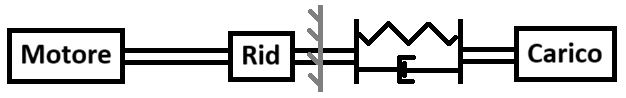
\includegraphics[width=0.5\textwidth]{Immagini/schema_antirisonanza.png}
    \caption{Schema equivalente per verifica su antirisonanza}
\end{figure}

\paragrafo{Relazione poli-zeri Gvm:}
Ricordando rapporto di inerzia \(\rho = \frac{\tau_R^2 J_c}{J_m} > 0\), in \(G_{vm}(s)\) esiste una relazione tra pulsazione del polo e pulsazione dello zero e per smorzamento del polo e smorzamento dello zero:
\[
\begin{cases}
    \omega_p = \omega_z \sqrt{1+\rho} \\
    \xi_p = \xi_z \sqrt{1+\rho} \\
    \omega_z < \omega_p \\
    \xi_z < \xi_p
\end{cases}
\]

\begin{figure}[h]
    \centering
    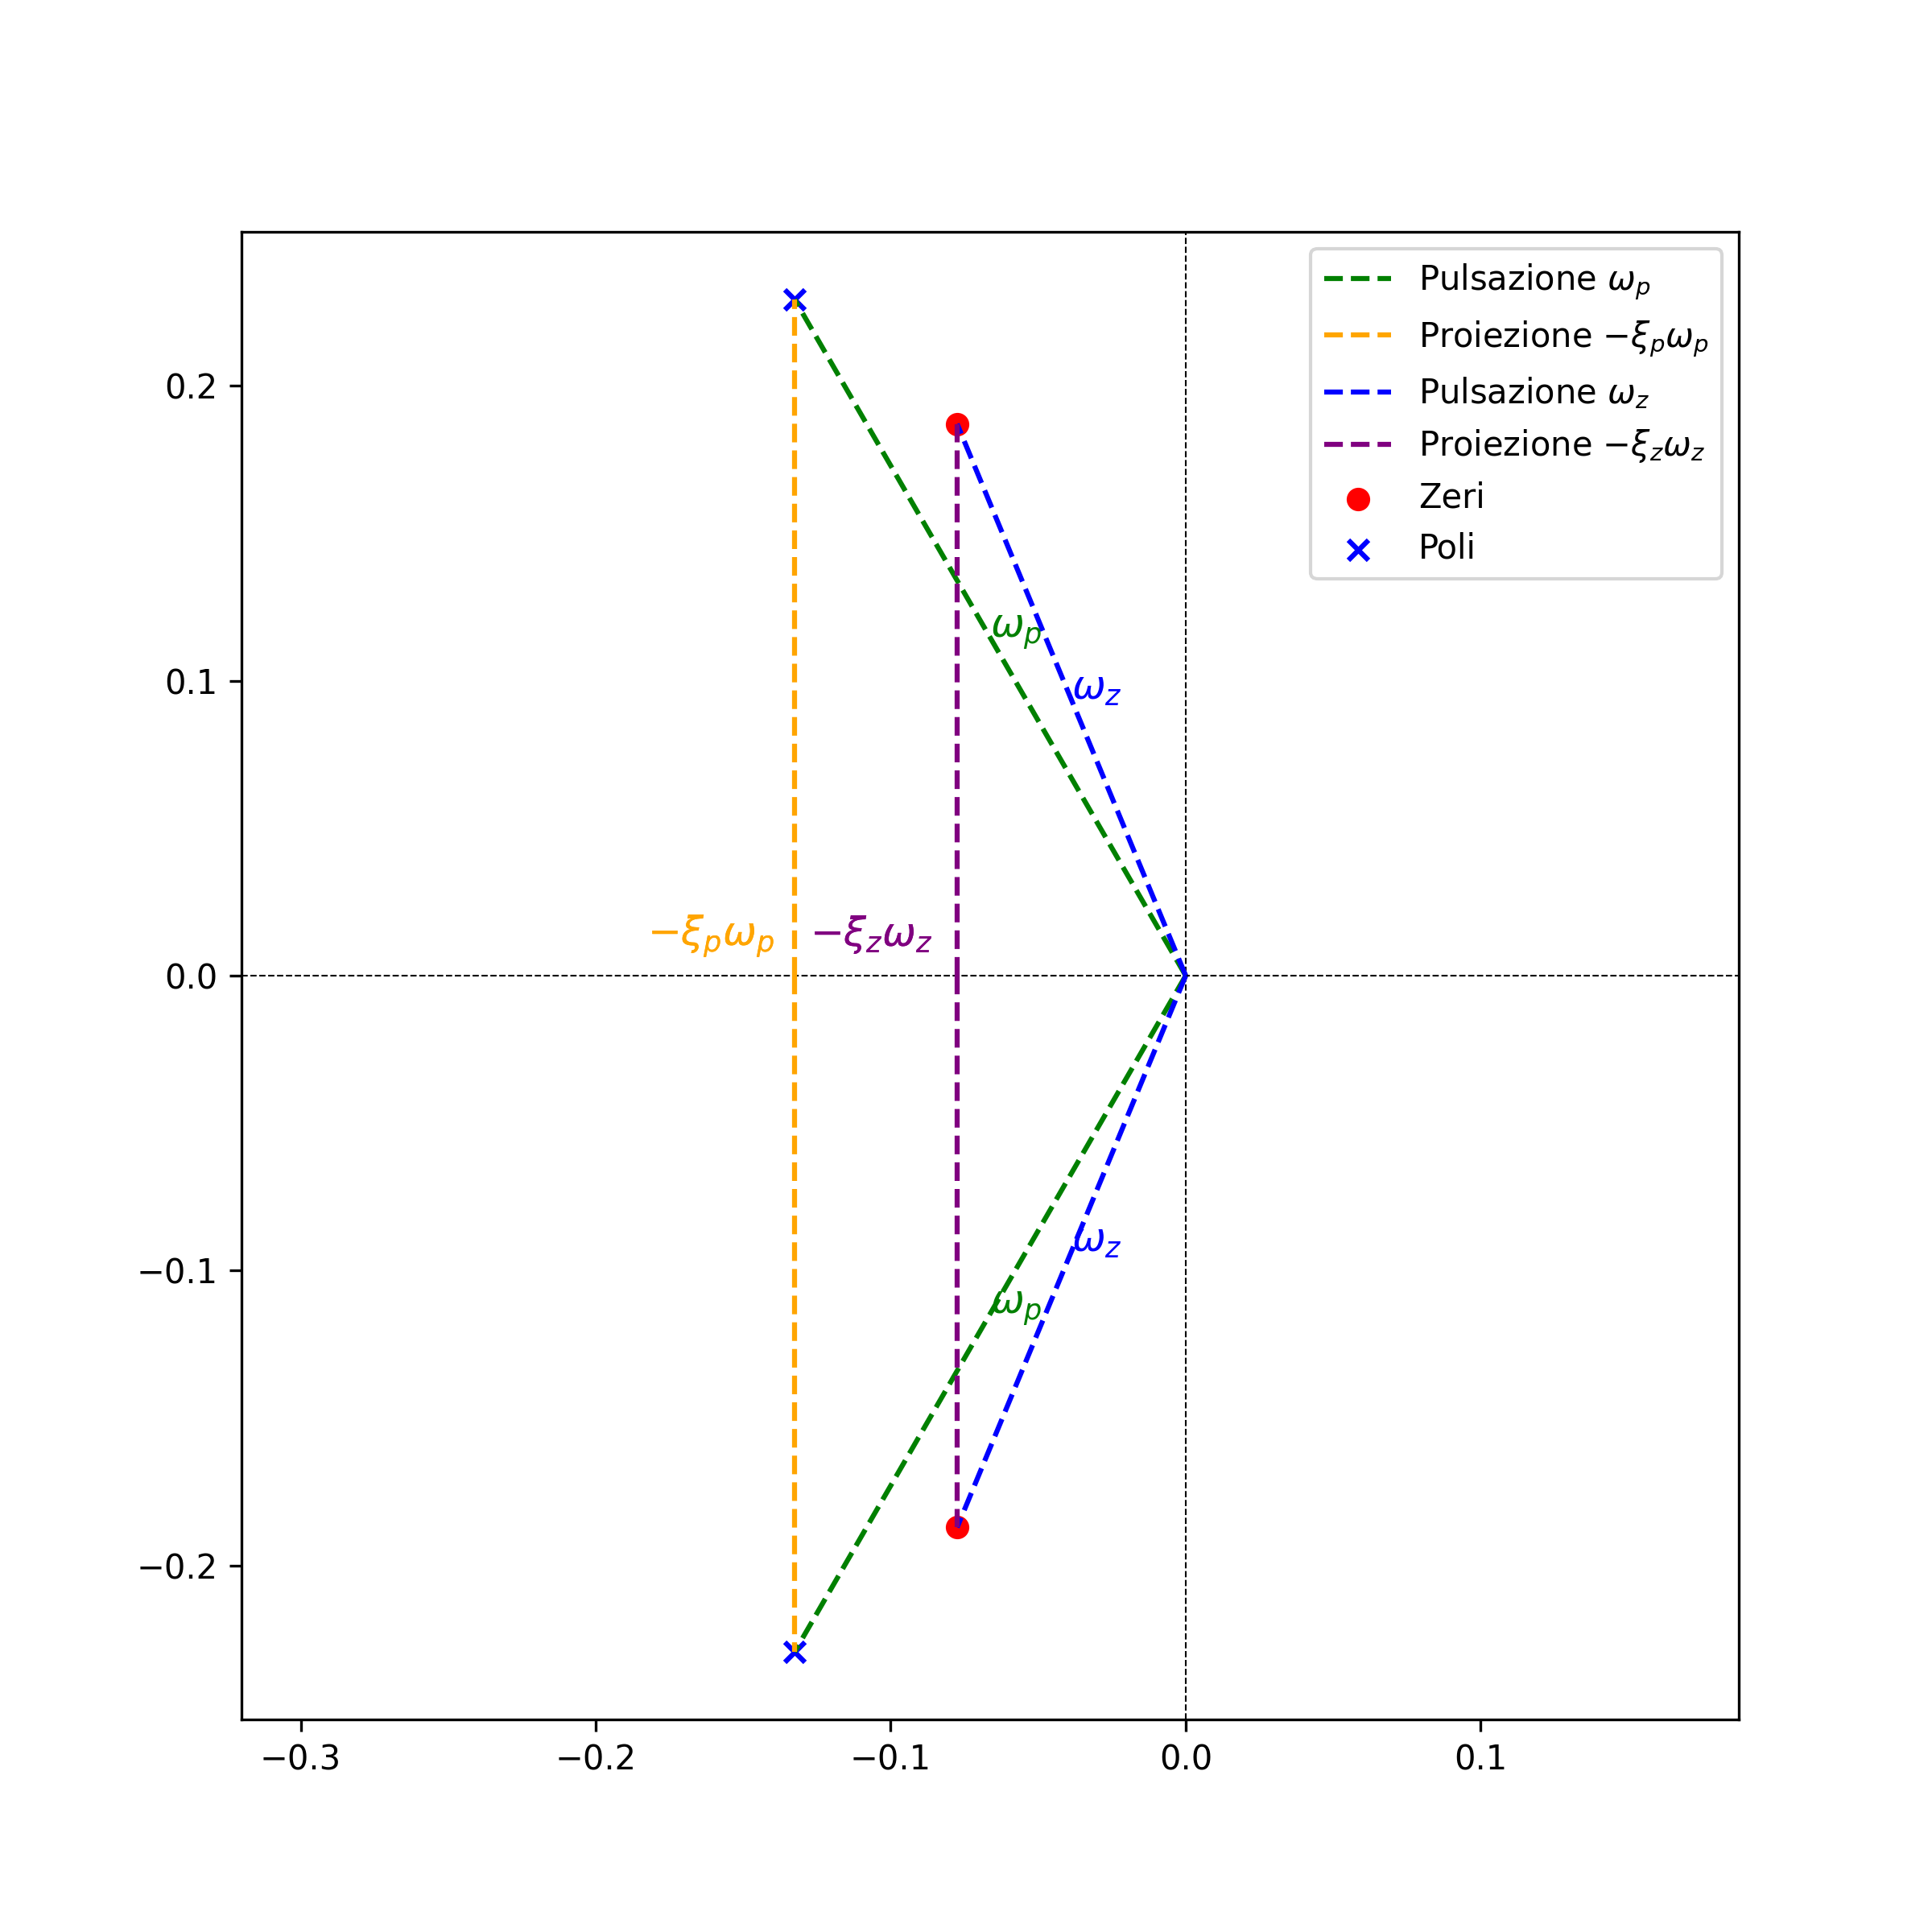
\includegraphics[width=0.5\textwidth]{Immagini/poli_zeri_Gvm.png}
    \caption{Rappresentazione su piano complesso di poli e zeri di \(G_{vm}\)}
\end{figure}

\sezione{Architetture di controllo}
Ci sono diverse tipologie di controllo in base alla grandezza misurata (o stimata) e grandezza attuata e se sono riferite entrambe allo stesso sitema (entrambe motore oppure una motore l'altra carico) o all'utilizzo di controllo SISO o MIMO.

\paragrafo{Controllo Co-Locato:}
Con controllo co-locato si intende un controllo in cui misura e grandezza attuata sono al motore; il carico si trova all'esterno del loop ed è in catena aperta.

\import{Immagini}{controllo_co_locato}

\paragrafo{Controllo non Co-Locato:}
Con controllo non co-locato si intende un controllo in cui misura e grandezza attuata sono differenti, in particolare la misura è effettuata al carico mentre la grandezza attuata è al motore; il carico si trova all'interno del loop.

\import{Immagini}{controllo_non_co_locato}

\paragrafo{Controllo di stato:}
Nel controllo di stato, lavorando in MIMO, permette di scegliere entrambe le grandezza di misura, risultando in un controllo migliore. Tuttavia nell'industria sono solitamente difficilmente praticabili. 

\sottosezione{Controllo Co-Locato vs non Co-Locato}
Per valutare quale controllo utilizzare vado a studiare intanto il controllo Co-Locato e in particolare l'inertanza (per semplicità di analisi) \(sG_{vm}(s)\) e la mobilità \(G_{vm}(s)\). Per il tracciamento si consiglia di studiare gli asintoti e quindi tracciare la funzione di trasferimento collegandoli.
Si notano in particolare \(m_\phi > 90^°\) e, non arrivando mai a \(-180^°\), vale anche \(m_a = \infty\). Questo è un ottimo segnale in termini di stabilità del sistema.

\begin{figure}[h]
    \centering
    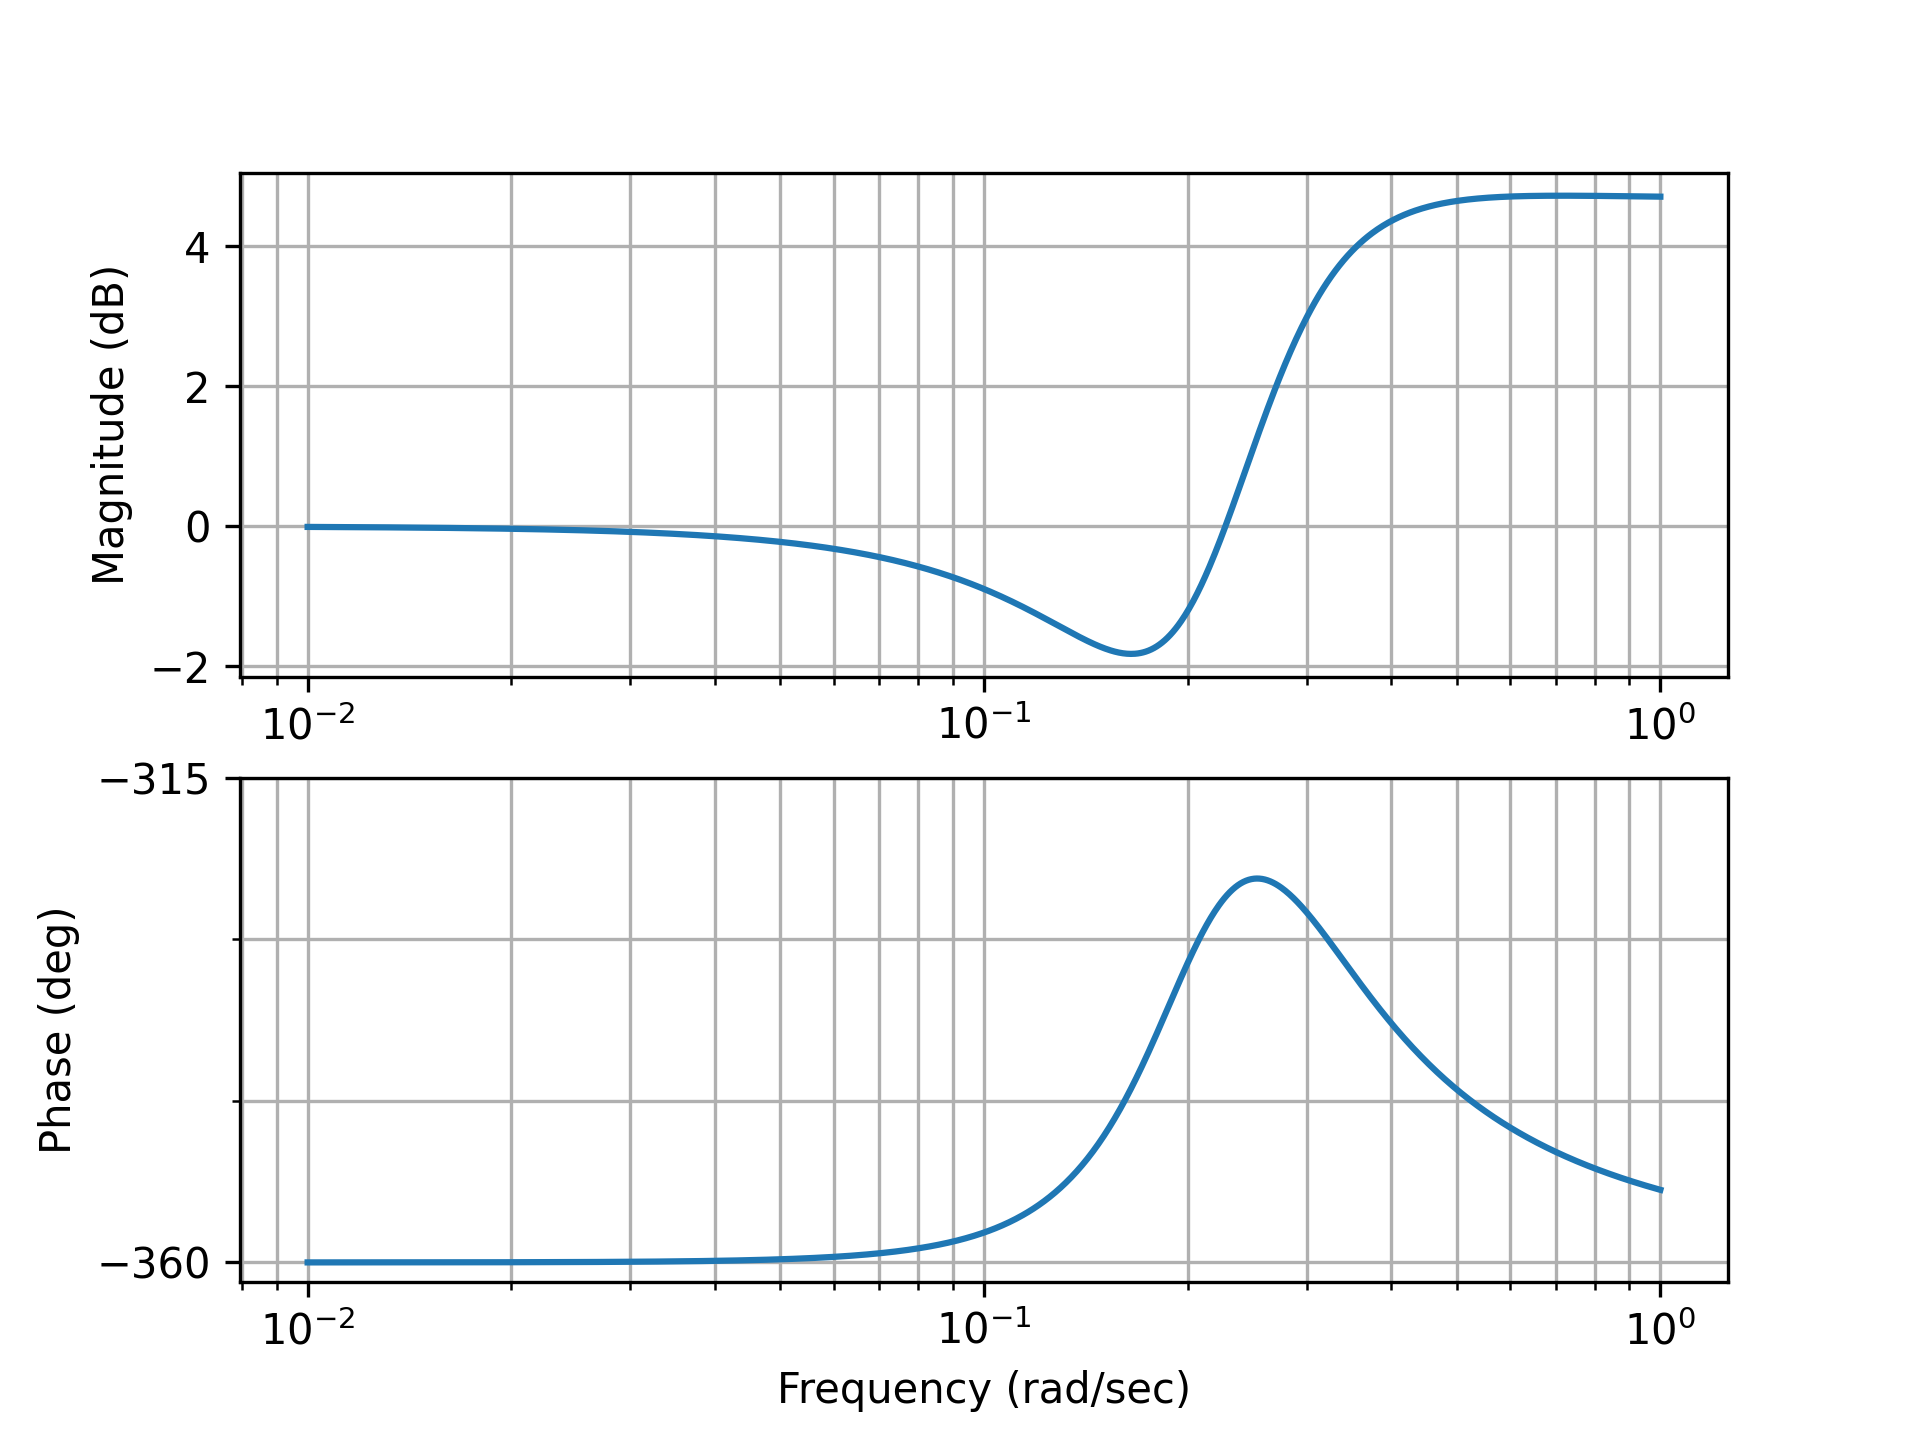
\includegraphics[width=0.45\textwidth]{Immagini/Inertanza_gvm.png}
    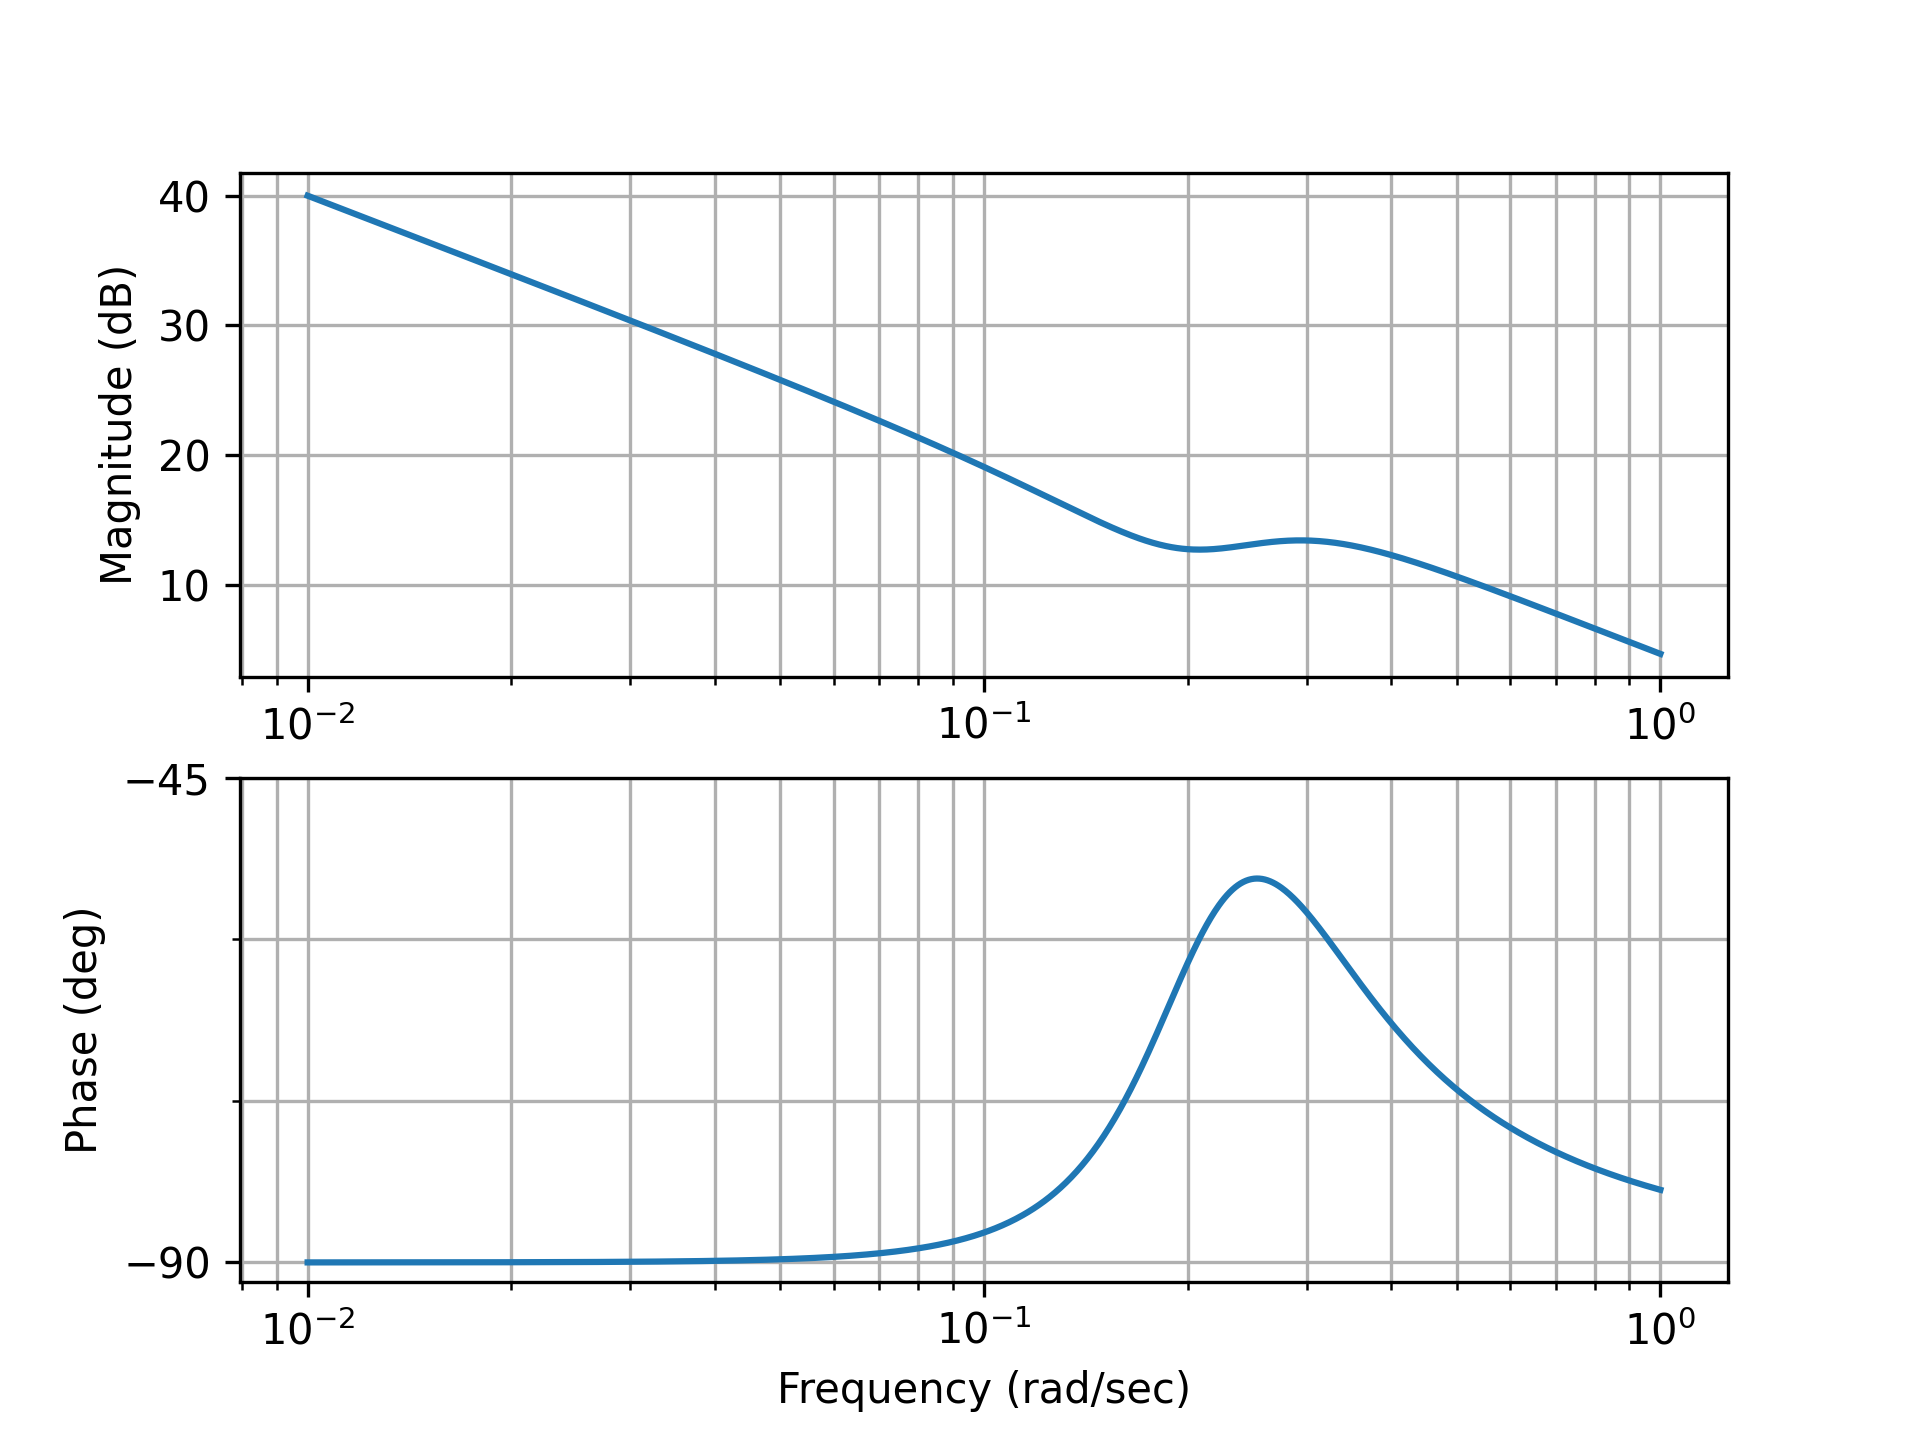
\includegraphics[width=0.45\textwidth]{Immagini/mobilita_gvm.png}
    \caption{Inertanza \(sG_{vm}\) sx e mobilità \(G_{vm}\)}
\end{figure}

\paragrafo{Controllo non Co-Locato:}
Per quanto riguarda il controllo non Co-Locato, facendo lo stesso ci si accorge di come la mobilità, complessivamente sia un sistema con polo del secondo ordine, inoltre il polo agisce prima dello zero, quindi in un certo tratto la fase potrebbe andare al di sotto dei \(-180^°\). Come risulta più chiaro dal grafico, questo aspetto ha conseguenze sulla stabilità del sistema: \textbf{Non si può fare un controllo non co-locato in velocità.}

\begin{figure}[h]
    \centering
    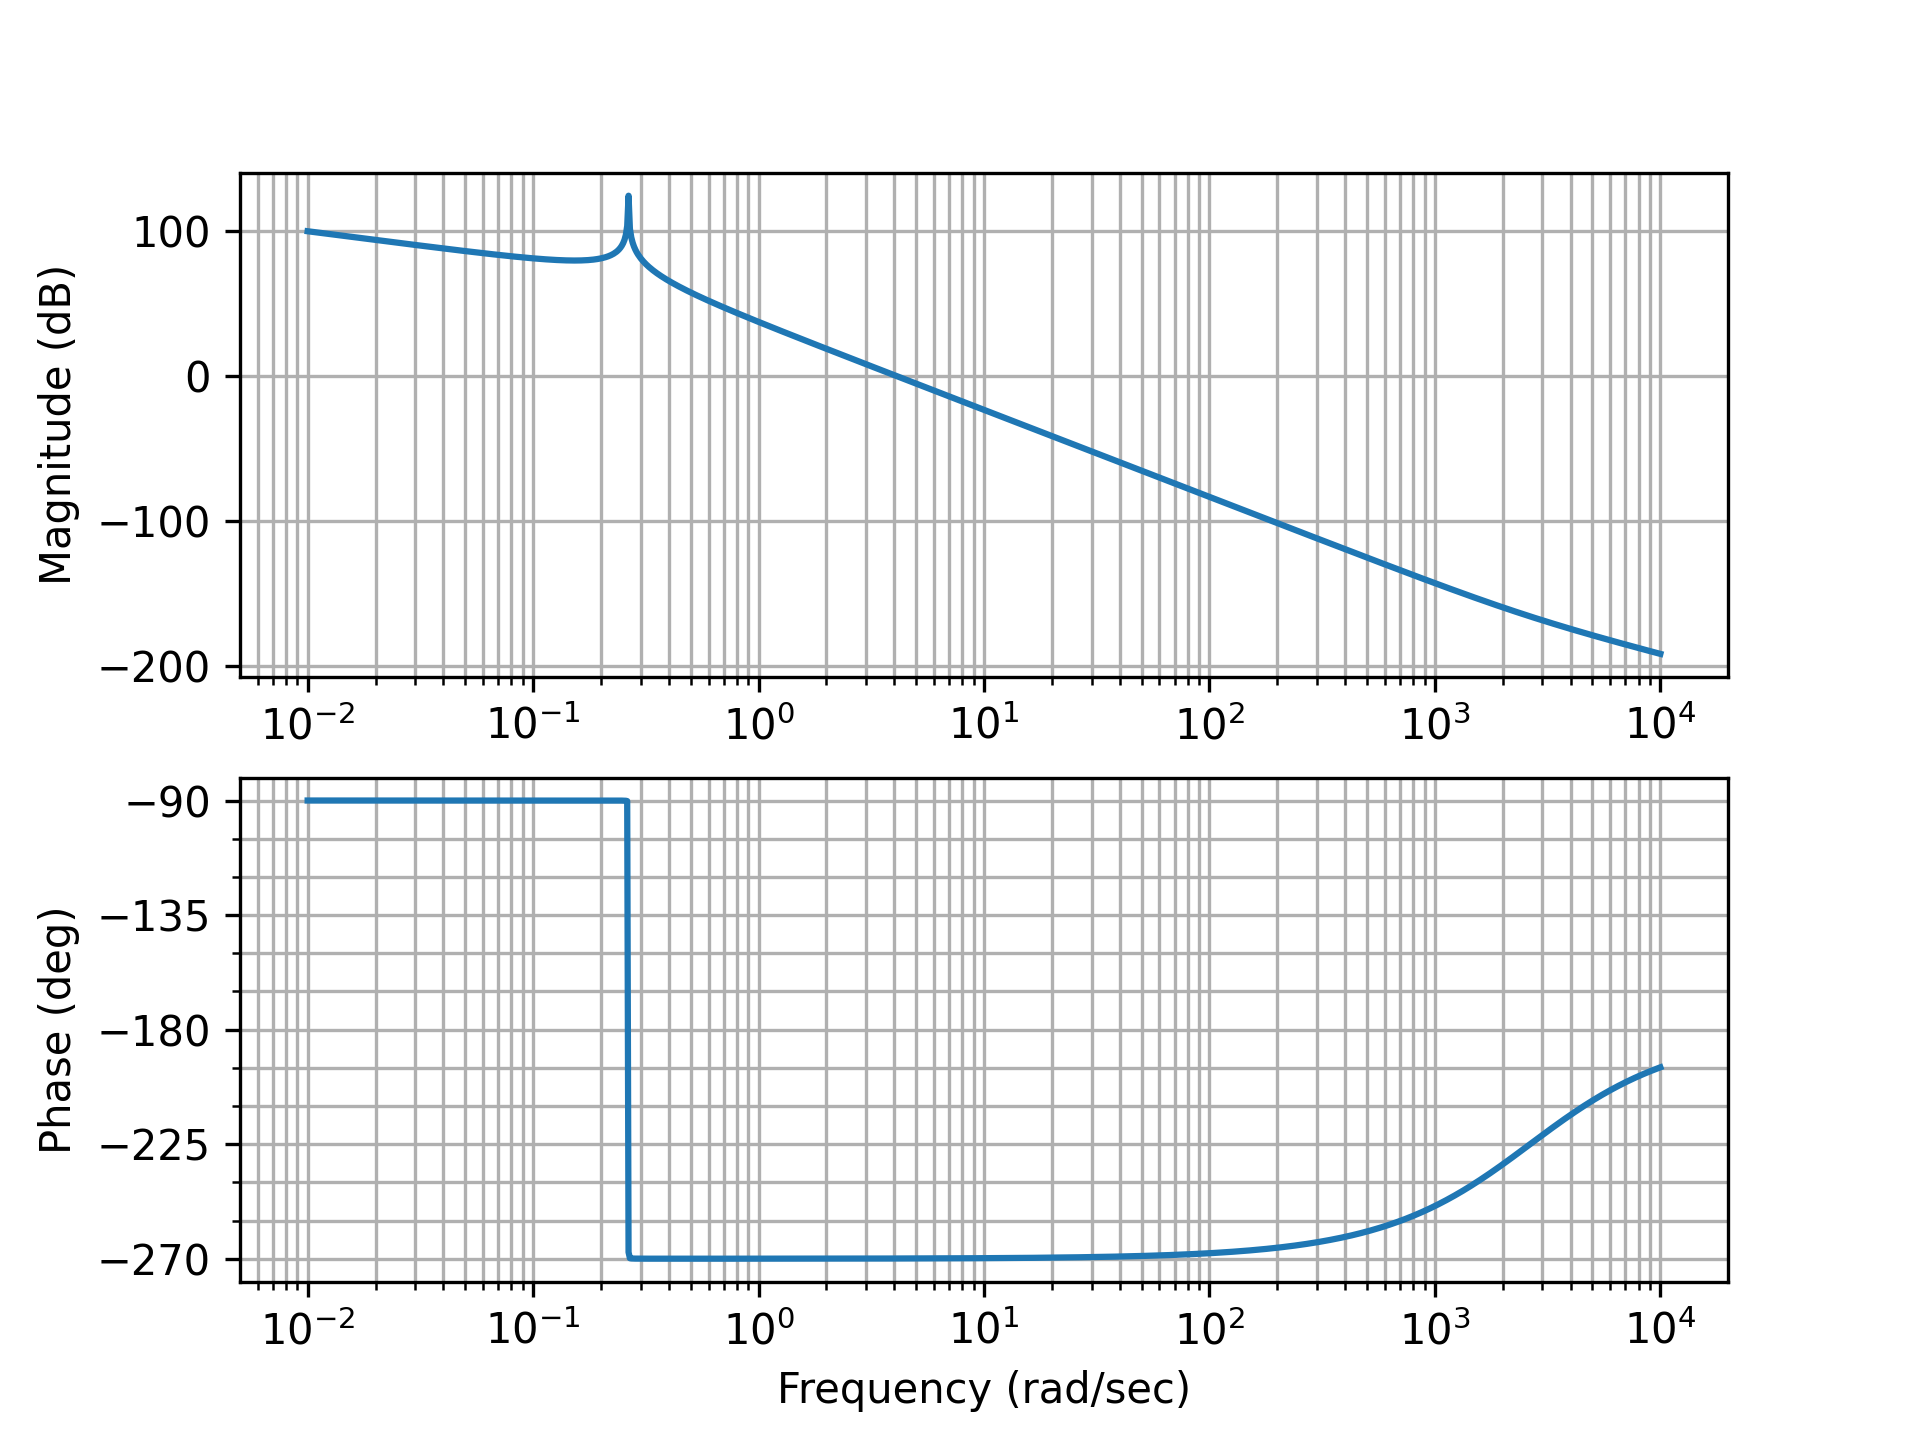
\includegraphics[width=0.45\textwidth]{Immagini/mobilita_gvc.png}
    \caption{Mobilità \(G_{vc}\)}
\end{figure}

\paragrafo{Luogo delle radici:}
Valutazioni simili possono essere fatte utilizzando il luogo delle radici\footnote{Vedi \ref{rlocus} per le regole di tracciamento, noi lavoreremo in modo qualitativo, quindi senza valutare esattamente gli asintoti, gli angoli di uscita o il passaggio per l'asse immaginario.}.

\begin{figure}[h]
    \centering
    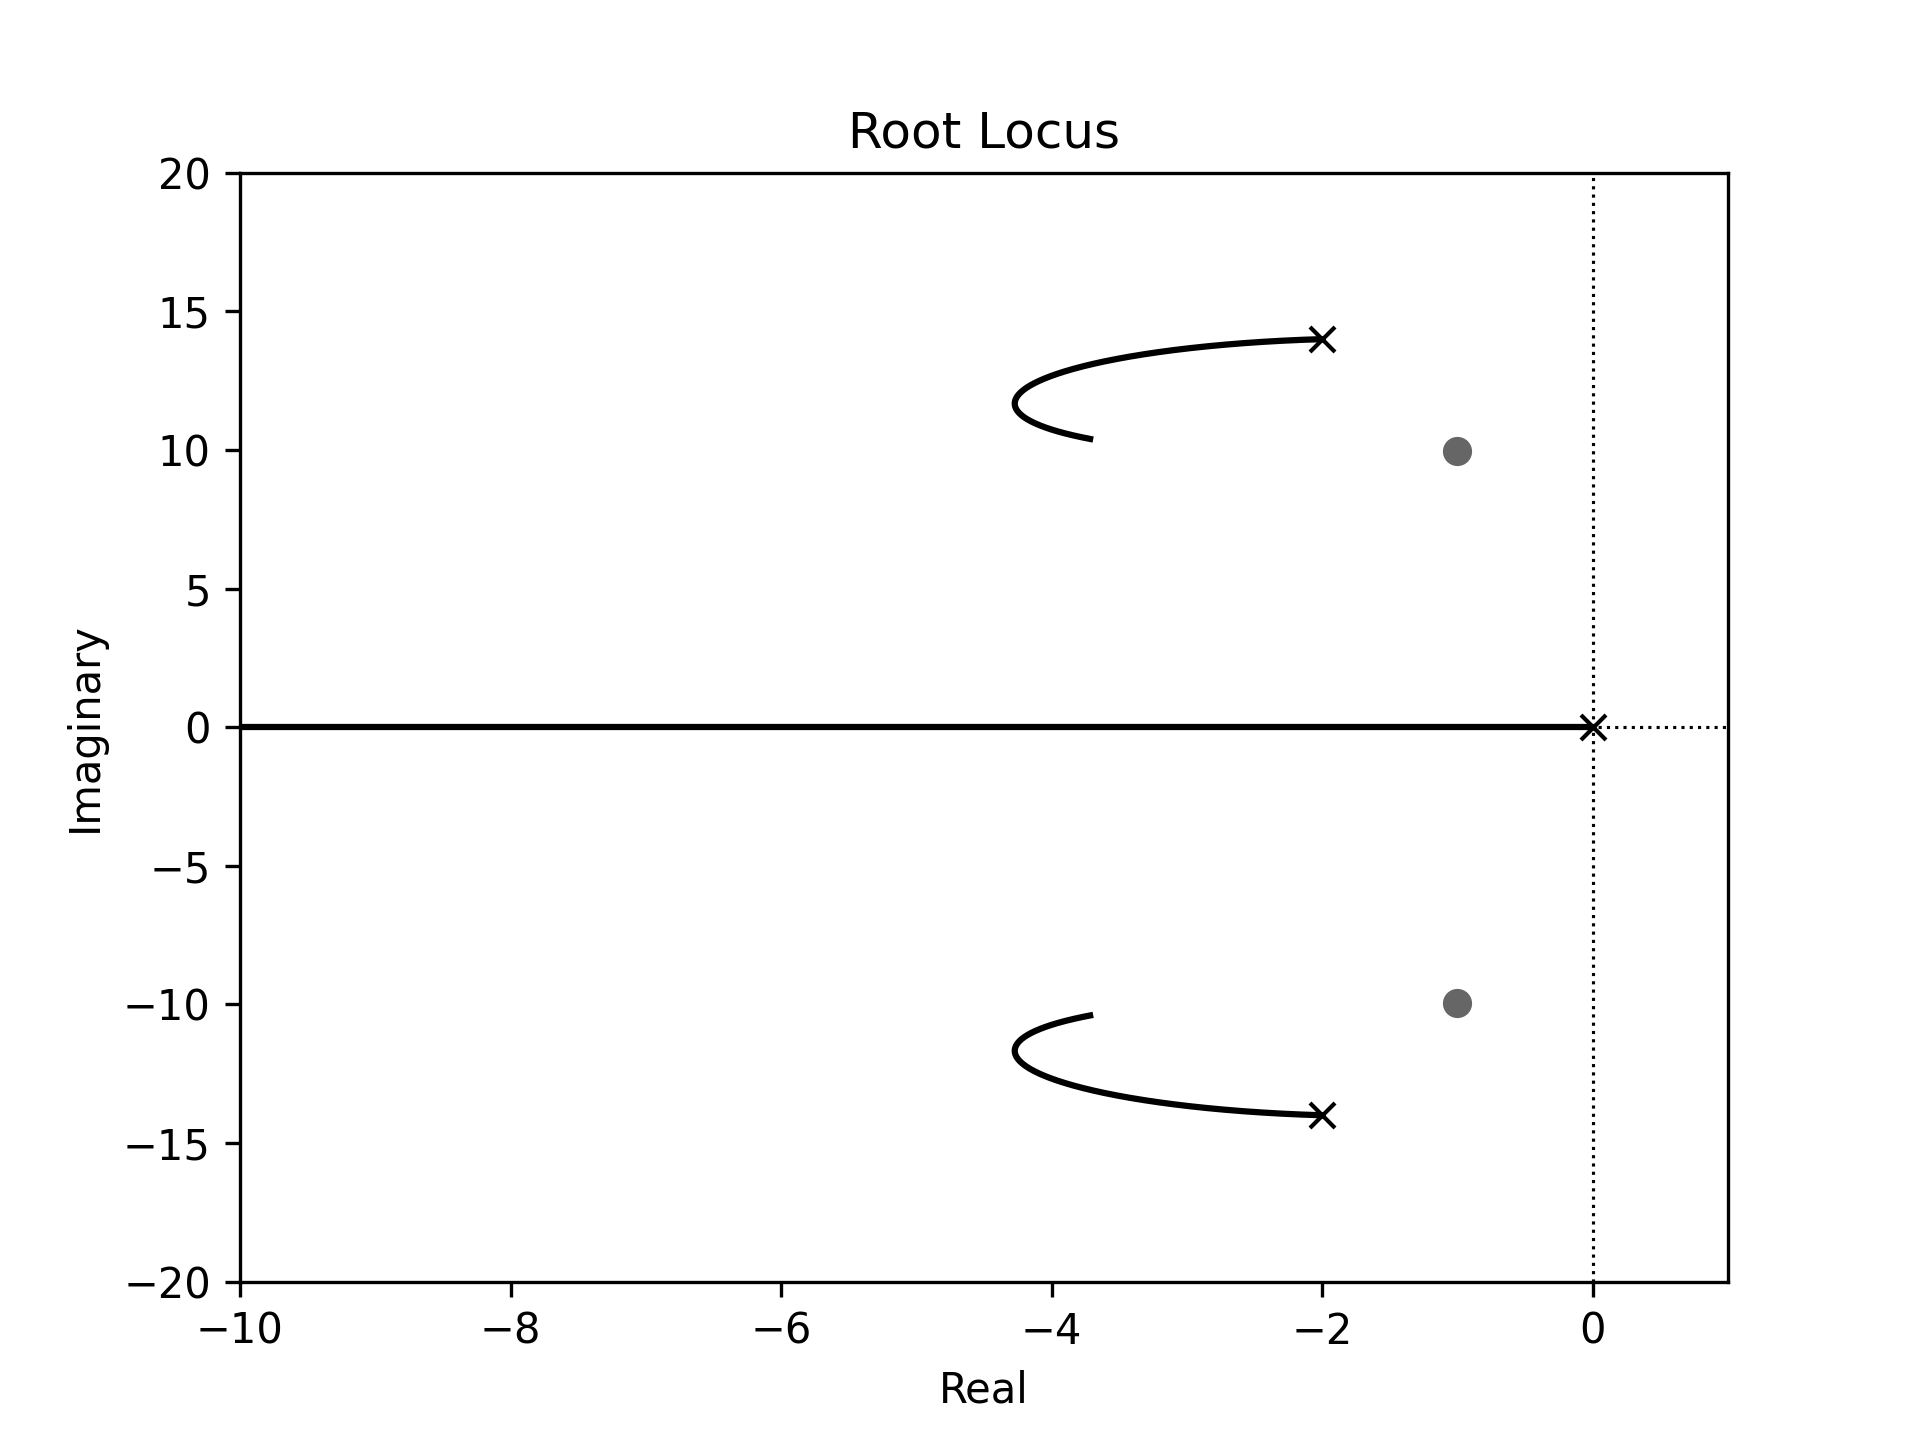
\includegraphics[width=0.45\textwidth]{Immagini/controllo_v_colocato.png}
    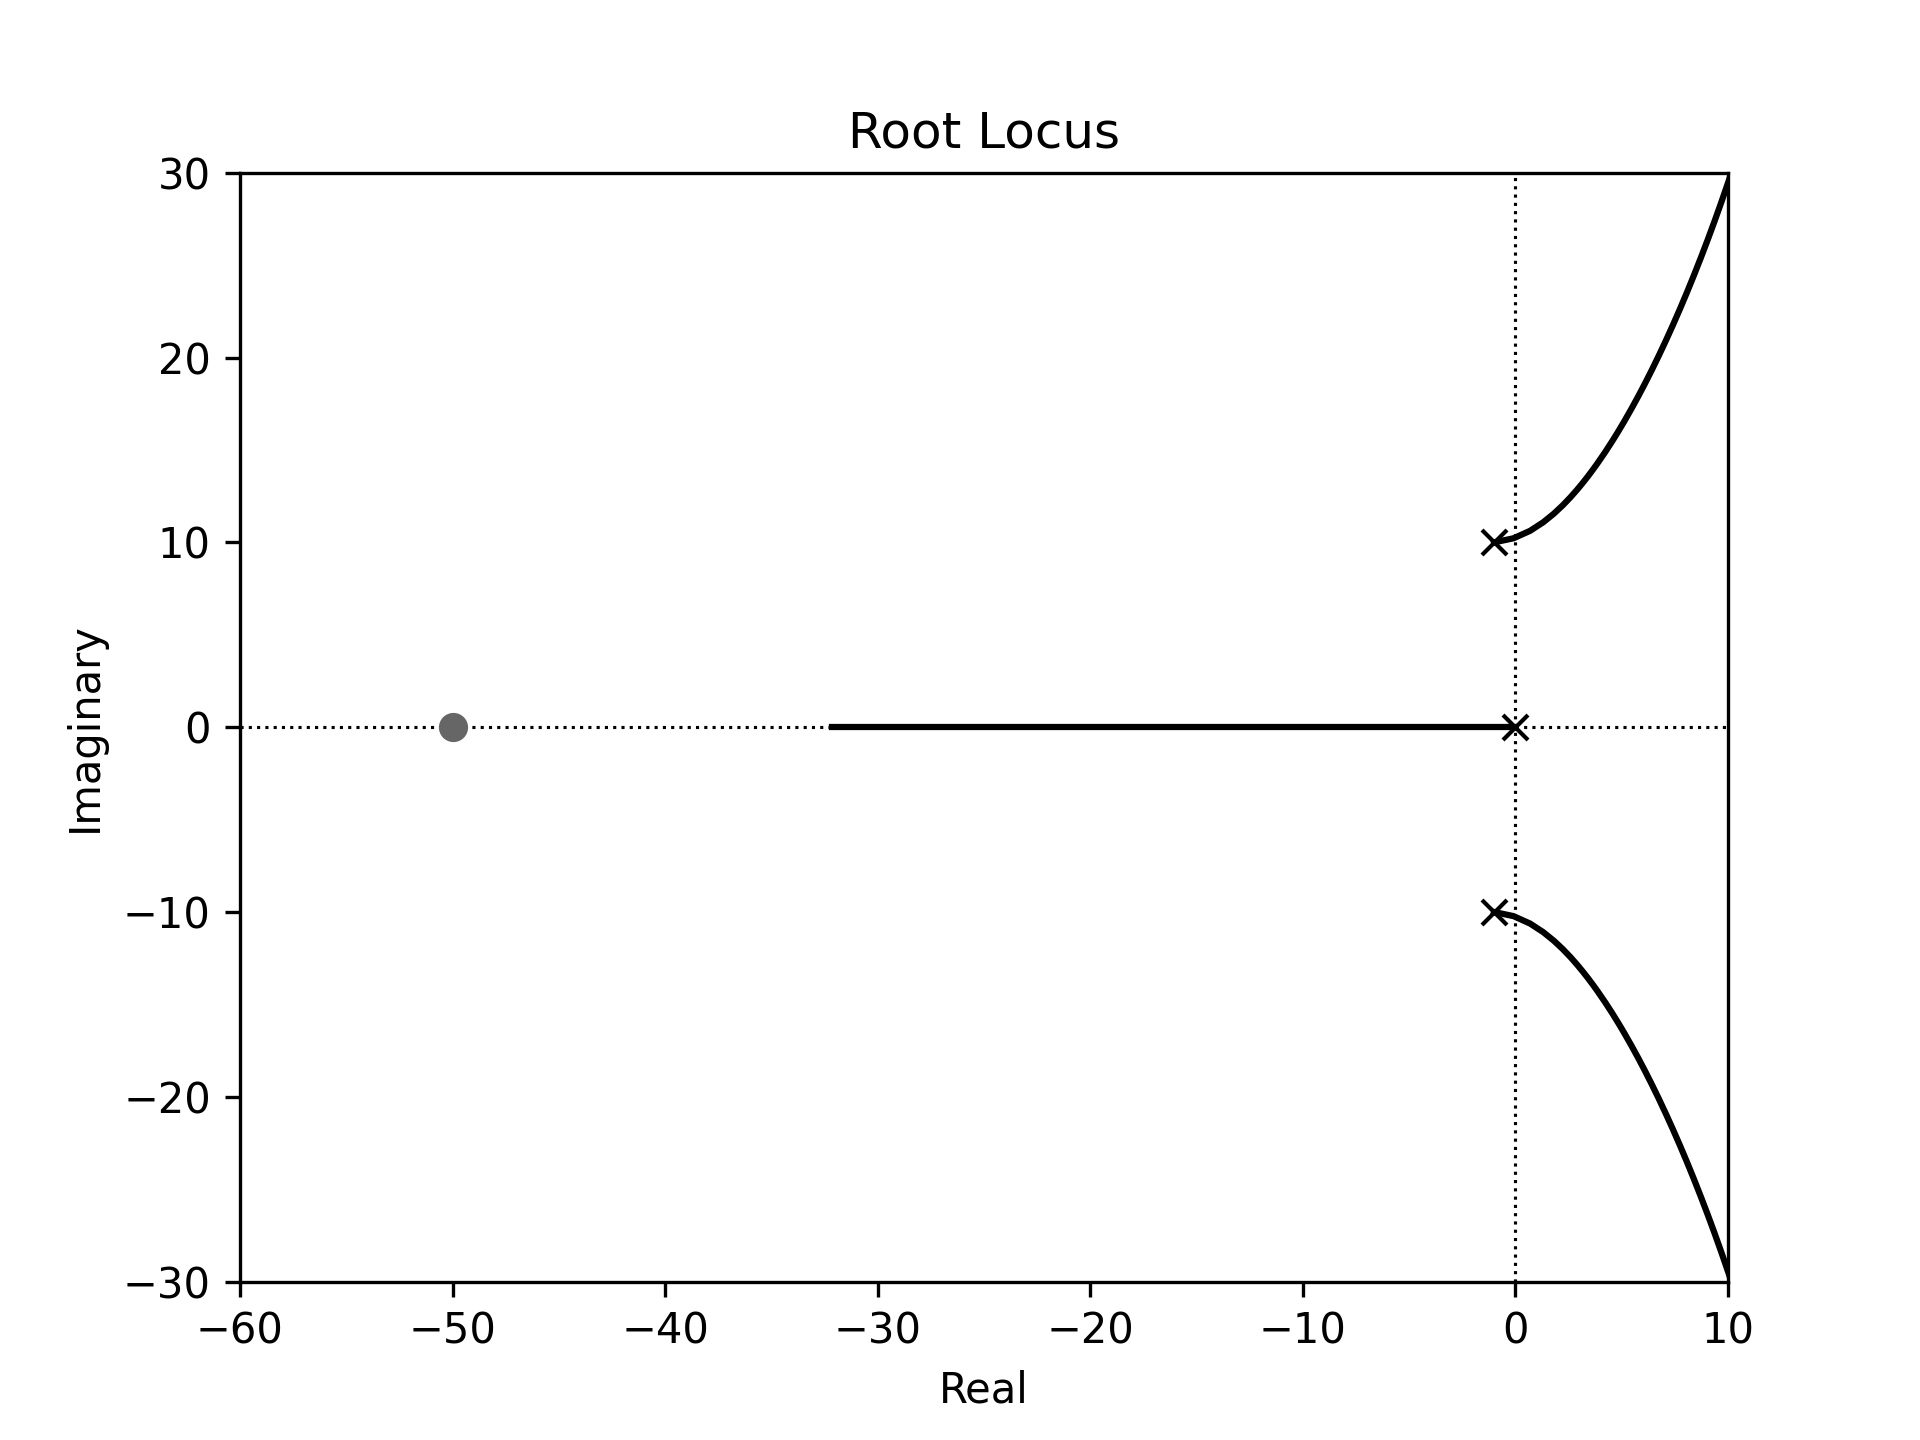
\includegraphics[width=0.45\textwidth]{Immagini/controllo_v_non_colocato.png}
    \caption{Controlli di velocità: Co-Locato sx; Non Co-Locato dx}
\end{figure}

\sottosezione{Trasmissibilità}
A completamento dell'analisi, si può studiare anche la trasmissibilità \(T(s) = \tau \frac{1+\frac{2\xi_z}{\omega_z}s}{1+\frac{2\xi_z}{\omega_z}s + \frac{s^2}{\omega_z^2}}\). Da notare come ad alta frequenza (come visto in Meccanica delle Vibrazioni) vi sia la zona di non trasmissione del moto, con modulo fortemente attenuato e ritardo. Il moto relativo di motore e carico è "grande".

\begin{figure}[h]
    \centering
    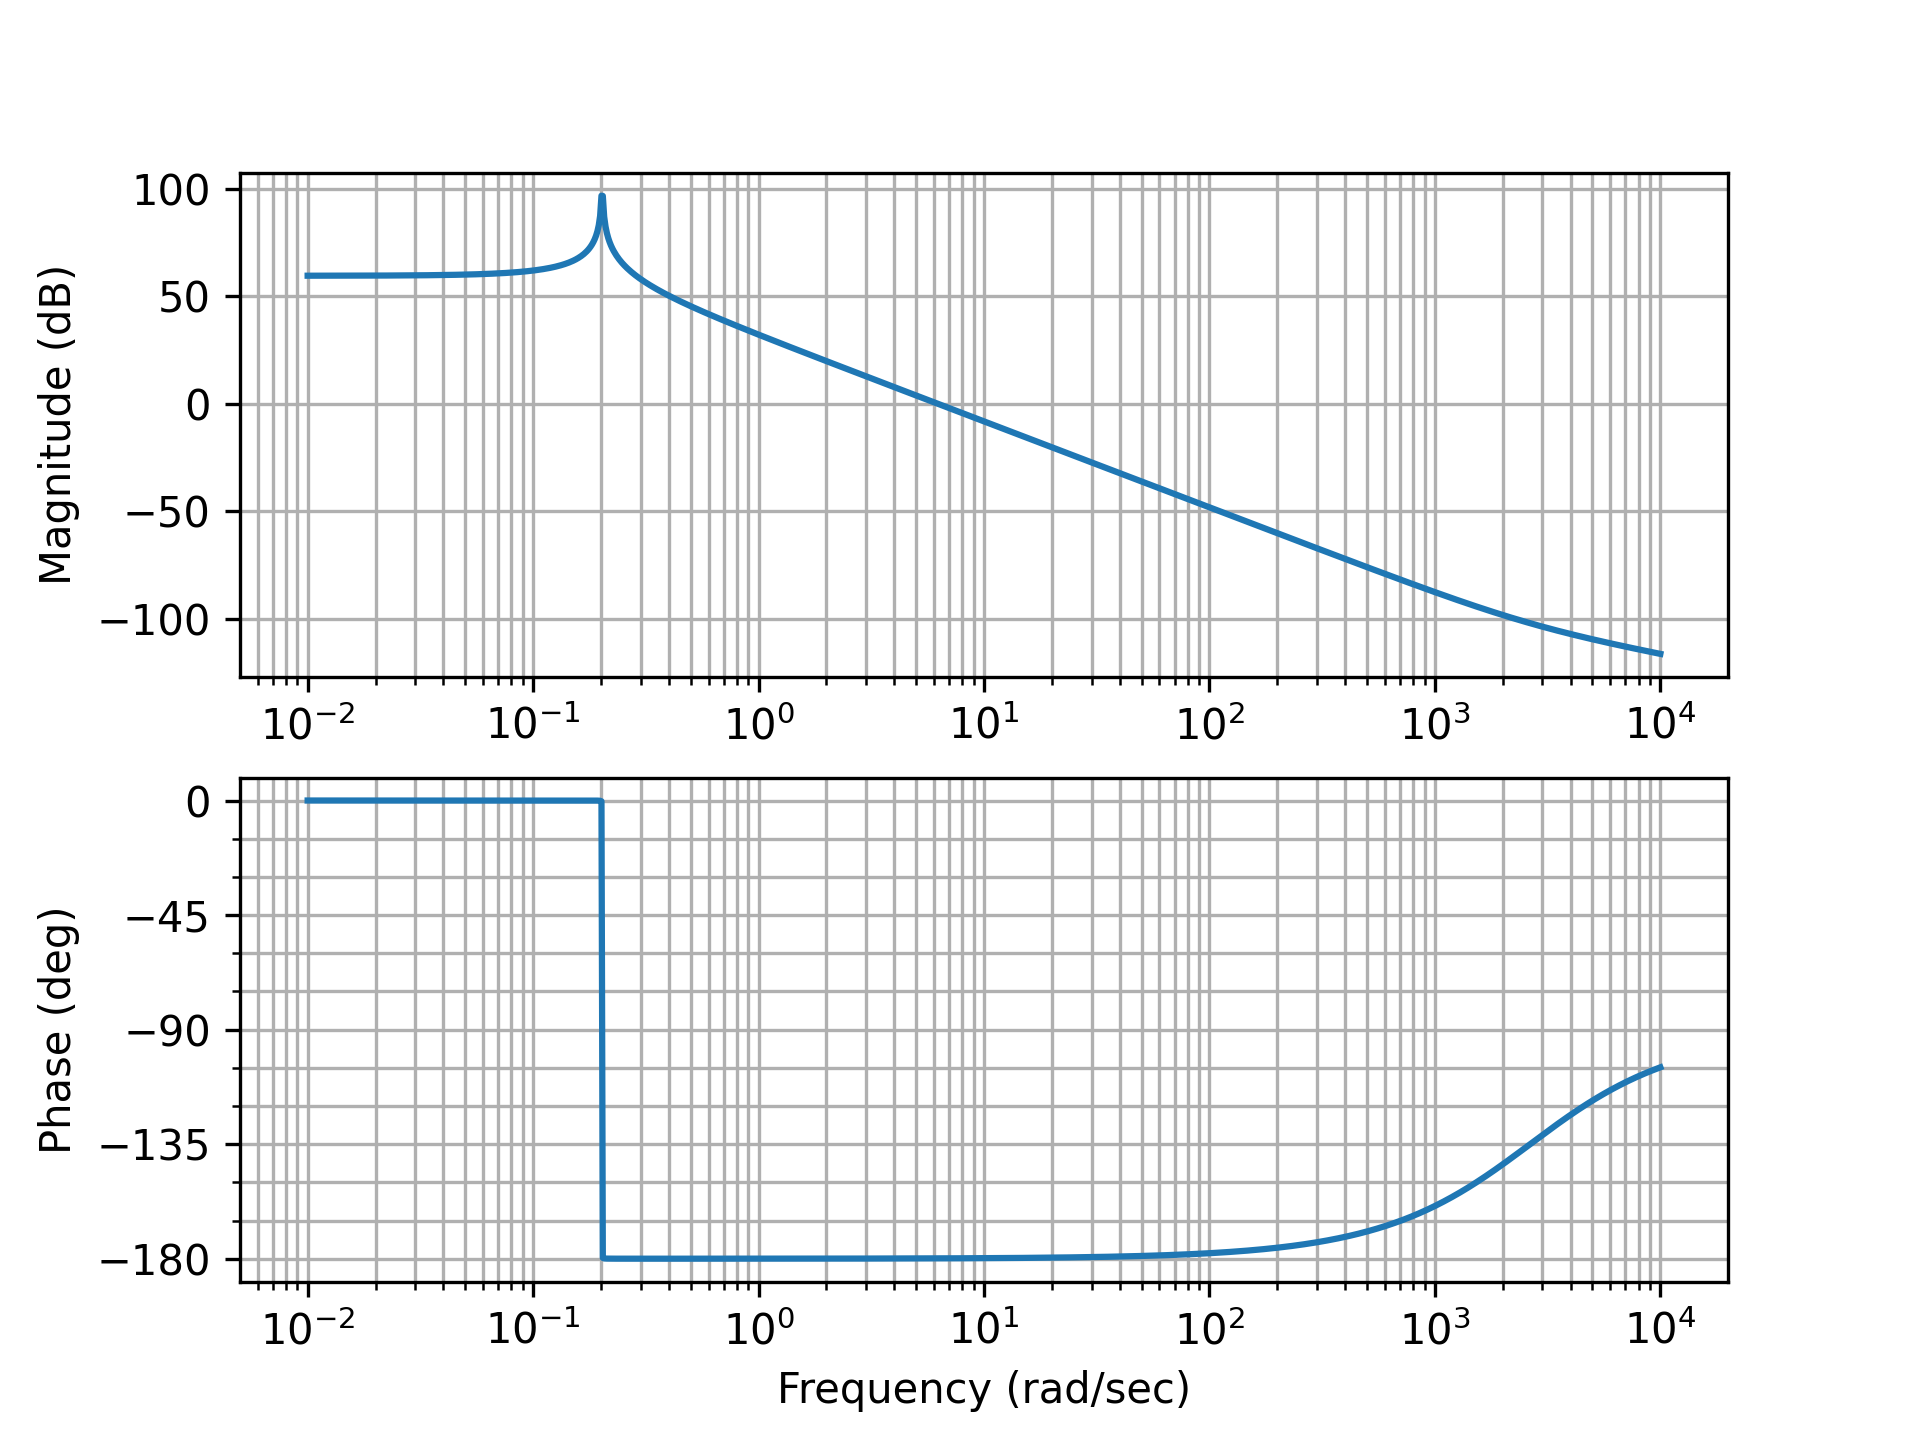
\includegraphics[width=0.45\textwidth]{Immagini/trasmissibilita.png}
    \caption{Trasmissibilità \(T(s)\)}
\end{figure}

\sottosezione{Attrito}
L'attrito ha implicazioni in tutto il sistema, volessi fare un'analisi rigorosa dovrei ricalcolare gli smorzamenti e le pulsazioni. Per un analisi approssimata invece è sufficiente considerare come l'attrito vada ad agire principalmente sul sistema rigido, quindi soprattutto per basse frequenze, si ottiene quindi il modello: \(G_{vm}(s) \simeq \frac{1}{sJ+f} \frac{\frac{s^2}{\omega_z^2} + \frac{2\xi_z}{\omega_z} s + 1}{\frac{s^2}{\omega_p^2} + \frac{2\xi_p}{\omega_p} s + 1}\). 

A differenza del precedente, al posto di avere un integrale in ingresso c'è un filtro passa basso, che in alta frequenza si comporta esattamente come un integrale.

In senso fisico, l'attrito è legato al moto assoluto (più rilevante in bassa frequenza), mentre l'attrito viscoso è maggiormente legato al moto relativo (più rilevante in alta frequenza).

\sottosezione{Controllo Co-Locato di Velocità}
Valutato come il controllo da utilizzare in velocità sia quello Co-Locato, considero due casi:
\[
\frac{\omega_p}{\omega_z} = \frac{\xi_p}{\xi_z} = \sqrt{1+\rho} \ \rightarrow \
\begin{cases}
    \rho \rightarrow 0 \text{ , allora } \omega_p\simeq \omega_z, \xi_p\simeq \xi_z \text{ cancellazione fisica polo-zero} \\
    \rho >> 0 \text{ , allora } \omega_p >> \omega_z, \xi_p >> \xi_z \text{ poli zeri ben distinti}
\end{cases}
\]


Dal luogo delle radici è possibile verificare come, col variare di \(K_{pv}\), varino: 
\begin{itemize}
    \item la lunghezza del vettore che collega origine e punti del luogo, che corrisponde alla variazione di pulsazione dei poli del sistema a catena chiusa \(W_v\)
    \item l'angolo del vettore, che corrisponde alla variazione di fattore di smorzamento del polo di \(W_v\)
    \item la proiezione del vettore sull'ascissa, che corrisponde a \(\abs{\mathbb{R}(W_v)}\)
\end{itemize}

\paragrafo{Significato fisico:}
\(\rho \simeq 1\) significa motore e carico di massa paragonabili. Il motore percepisce oscillazioni del carico, può quindi attivarsi per cercare di limitarle.
\(\rho \rightarrow 0\) significa motore di massa tanto maggiore a quella del carico. Il controllo viene visto come semplificato perché qualsiasi problematica di carico non viene percepita dal motore. Soluzione per questo caso è quella di utilizzare un controllo in controllo di stato (se possibile) oppure scegliere una legge di moto dolce standard o ad hoc (in particolare leggi di moto dolci ad hoc per \(\rho \rightarrow 0\) si vedranno in laboratorio).

\begin{figure}[h]
    \centering
    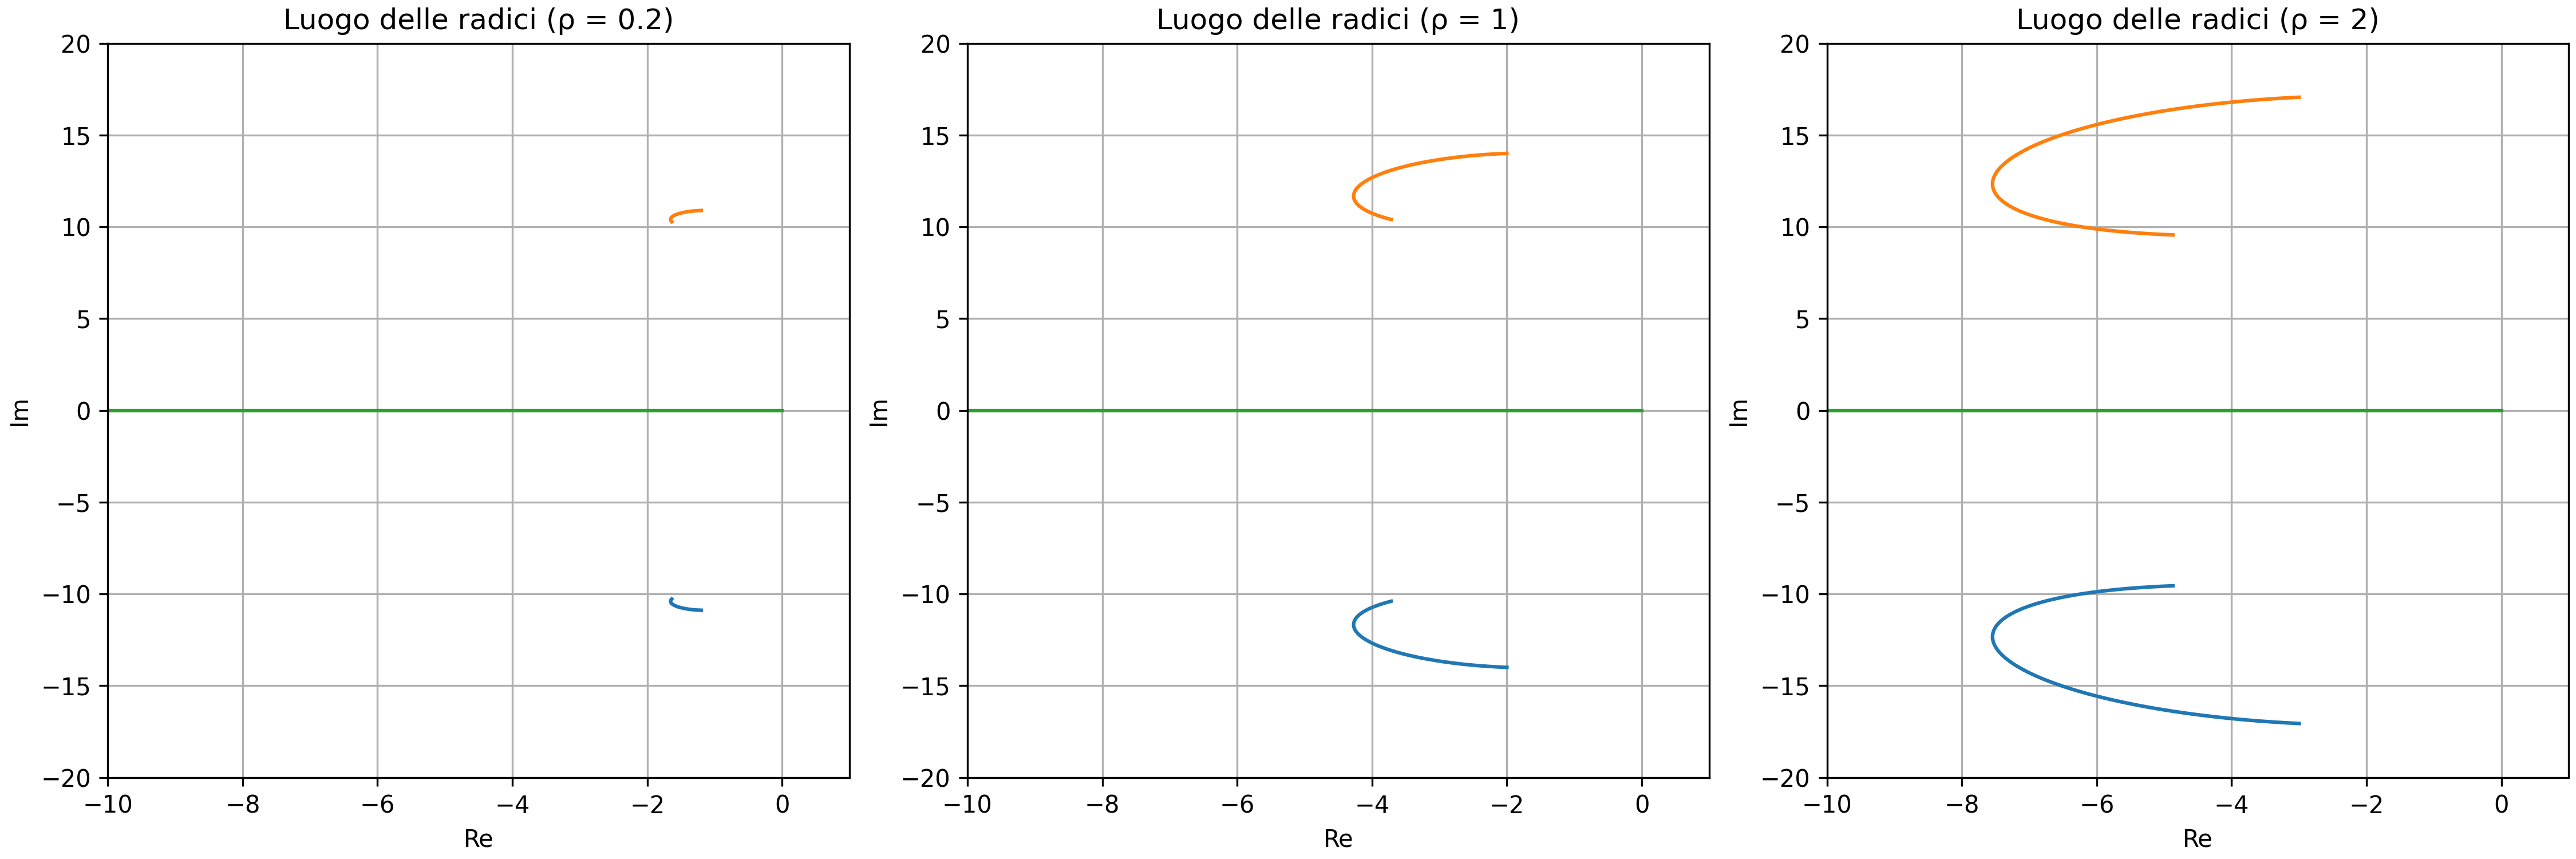
\includegraphics[width=0.8\textwidth]{Immagini/controllo_v_colocato_subplot_rho.png}
    \caption{Controllo Co-Locato per vari \(\rho\)}
\end{figure}

\paragrafo{Relazione smorzamento massimo di Wv e rho:}
Sussiste una relazione tra il massimo smorzamento dei poli di \(W_v\) e \(\rho\): \(\xi_{max} = \xi_p + \frac{\sqrt{1+\rho}}{2} - 1\). Questa relazione (non da sapere a memoria) evidenzia come lo smorzamento massimo dei poli di \(W_v\) sia maggiore di quello dei poli a catena aperta, ed è legato a quanto visto per il luogo delle radici in cui è evidente la dipendenza tra \(\rho\) e \(\alpha\).

\sottosottosezione{Rapporto di inerzia nullo}
Per \(\rho \rightarrow 0\) il controllo di motore è equivalente al controllo di un asse rigido, avente \(\omega_{bv}\) elevata. La banda elevata può portare ad avere il motore, se comandato con legge non dolce, ad eccitare il carico.

Considero l'errore di posizione al carico: \(e_c(t) = \theta_c^{des}(t) - \theta_c^{mis}(t)\) considerando \(\tau=1\), solo per semplificare il ragionamento, e \(\theta_c^{mis} = \theta_c\) ossia che il motore venga controllato bene (ipotesi realistica, considerando che sto lavorando con un equivalente asse rigido) \(e_c(t) = \theta_M^{des}(t) - \theta_c(t)\), passando in Laplace si ottiene \(E(s) = \theta_M (s) - \theta_c(s) = \theta_M(s) (1 - T(s)) = \theta_M(s) \frac{\frac{s^2}{\omega_z^2}}{\frac{s^2}{\omega_z^2} + \frac{2\xi_z}{\omega_z}s + 1}\), da cui si ottiene la formulazione:
\[
E(s) = \frac{A_M(s)}{\omega_z^2} \frac{1}{\frac{s^2}{\omega_z^2} + \frac{2\xi_z}{\omega_z}s + 1}
\]

In cui viene evidenziata la relazione tra errore in posizione motore-carico e accelerazione del motore. Questo ha conseguenze sulla scelta della legge di moto perché avere accelerazione maggiore (a parità di altro), è associato ad accelerazioni maggiore. Inoltre viene evidenziato l'effetto della pulsazione dello zero \(\omega_z\) che va ad abbattere l'errore di posizione.

\begin{figure}[h]
    \centering
    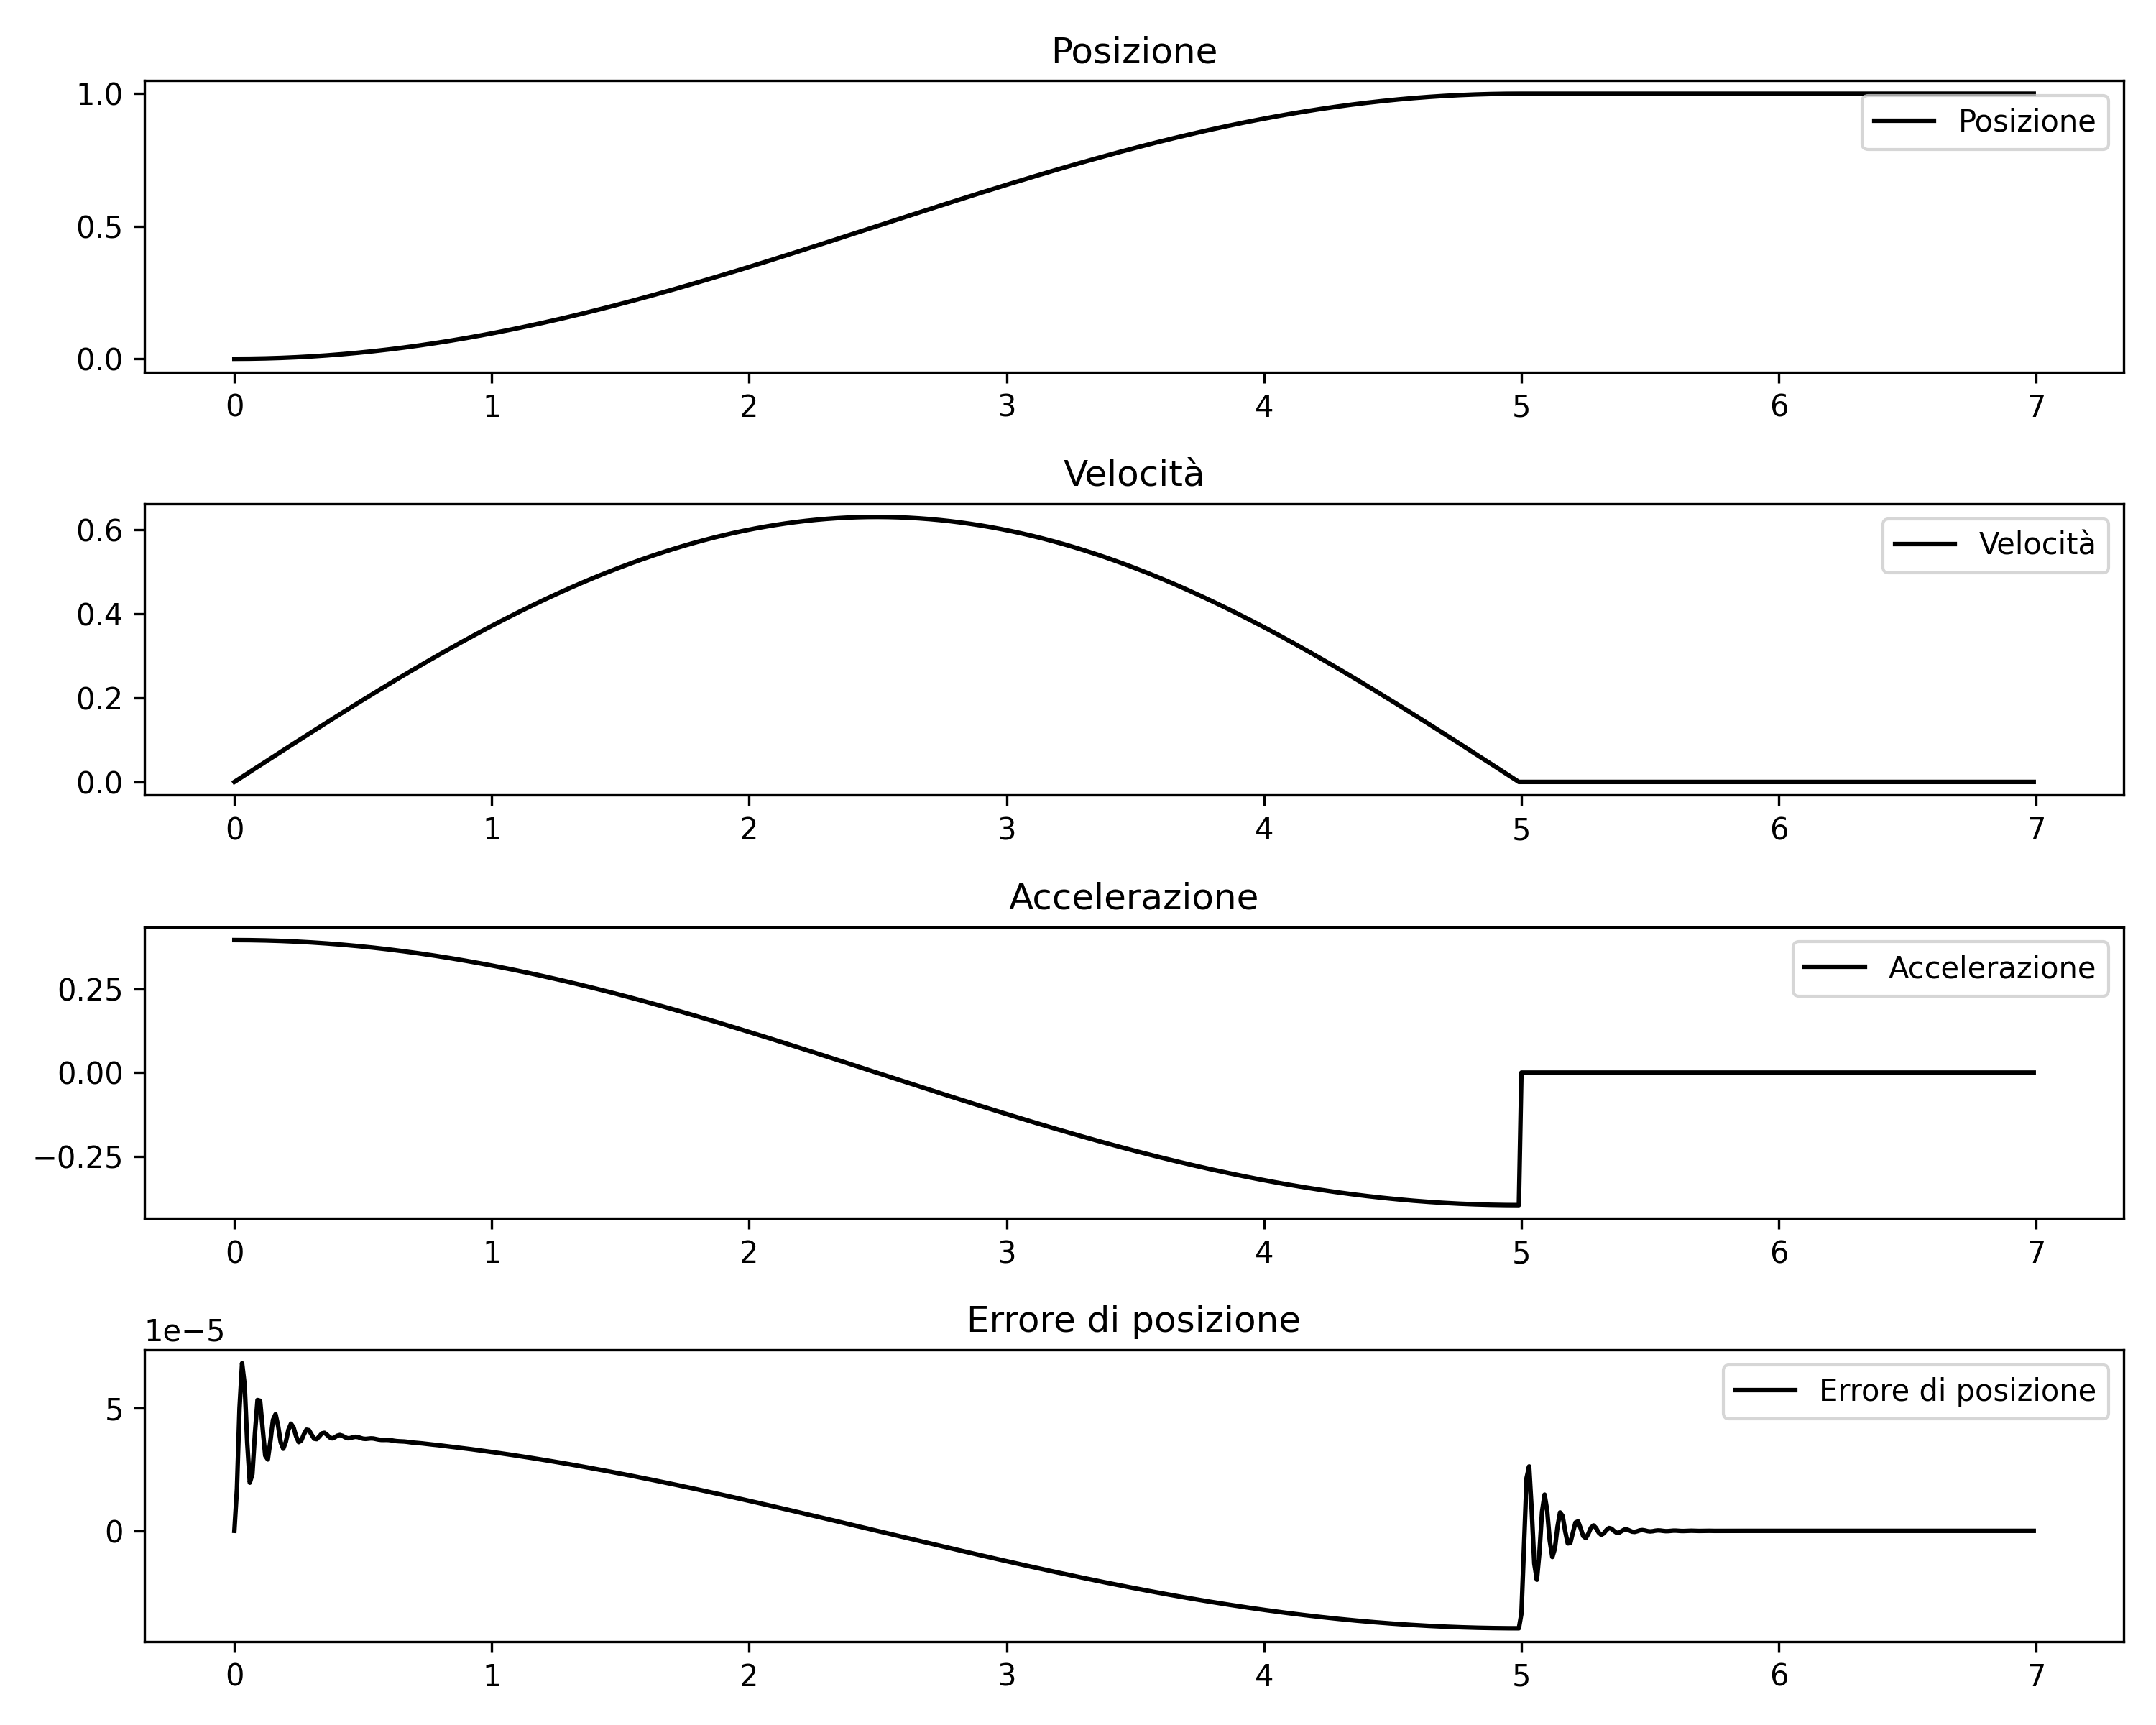
\includegraphics[width=0.45\textwidth]{Immagini/armonica_colocato_v.png}
    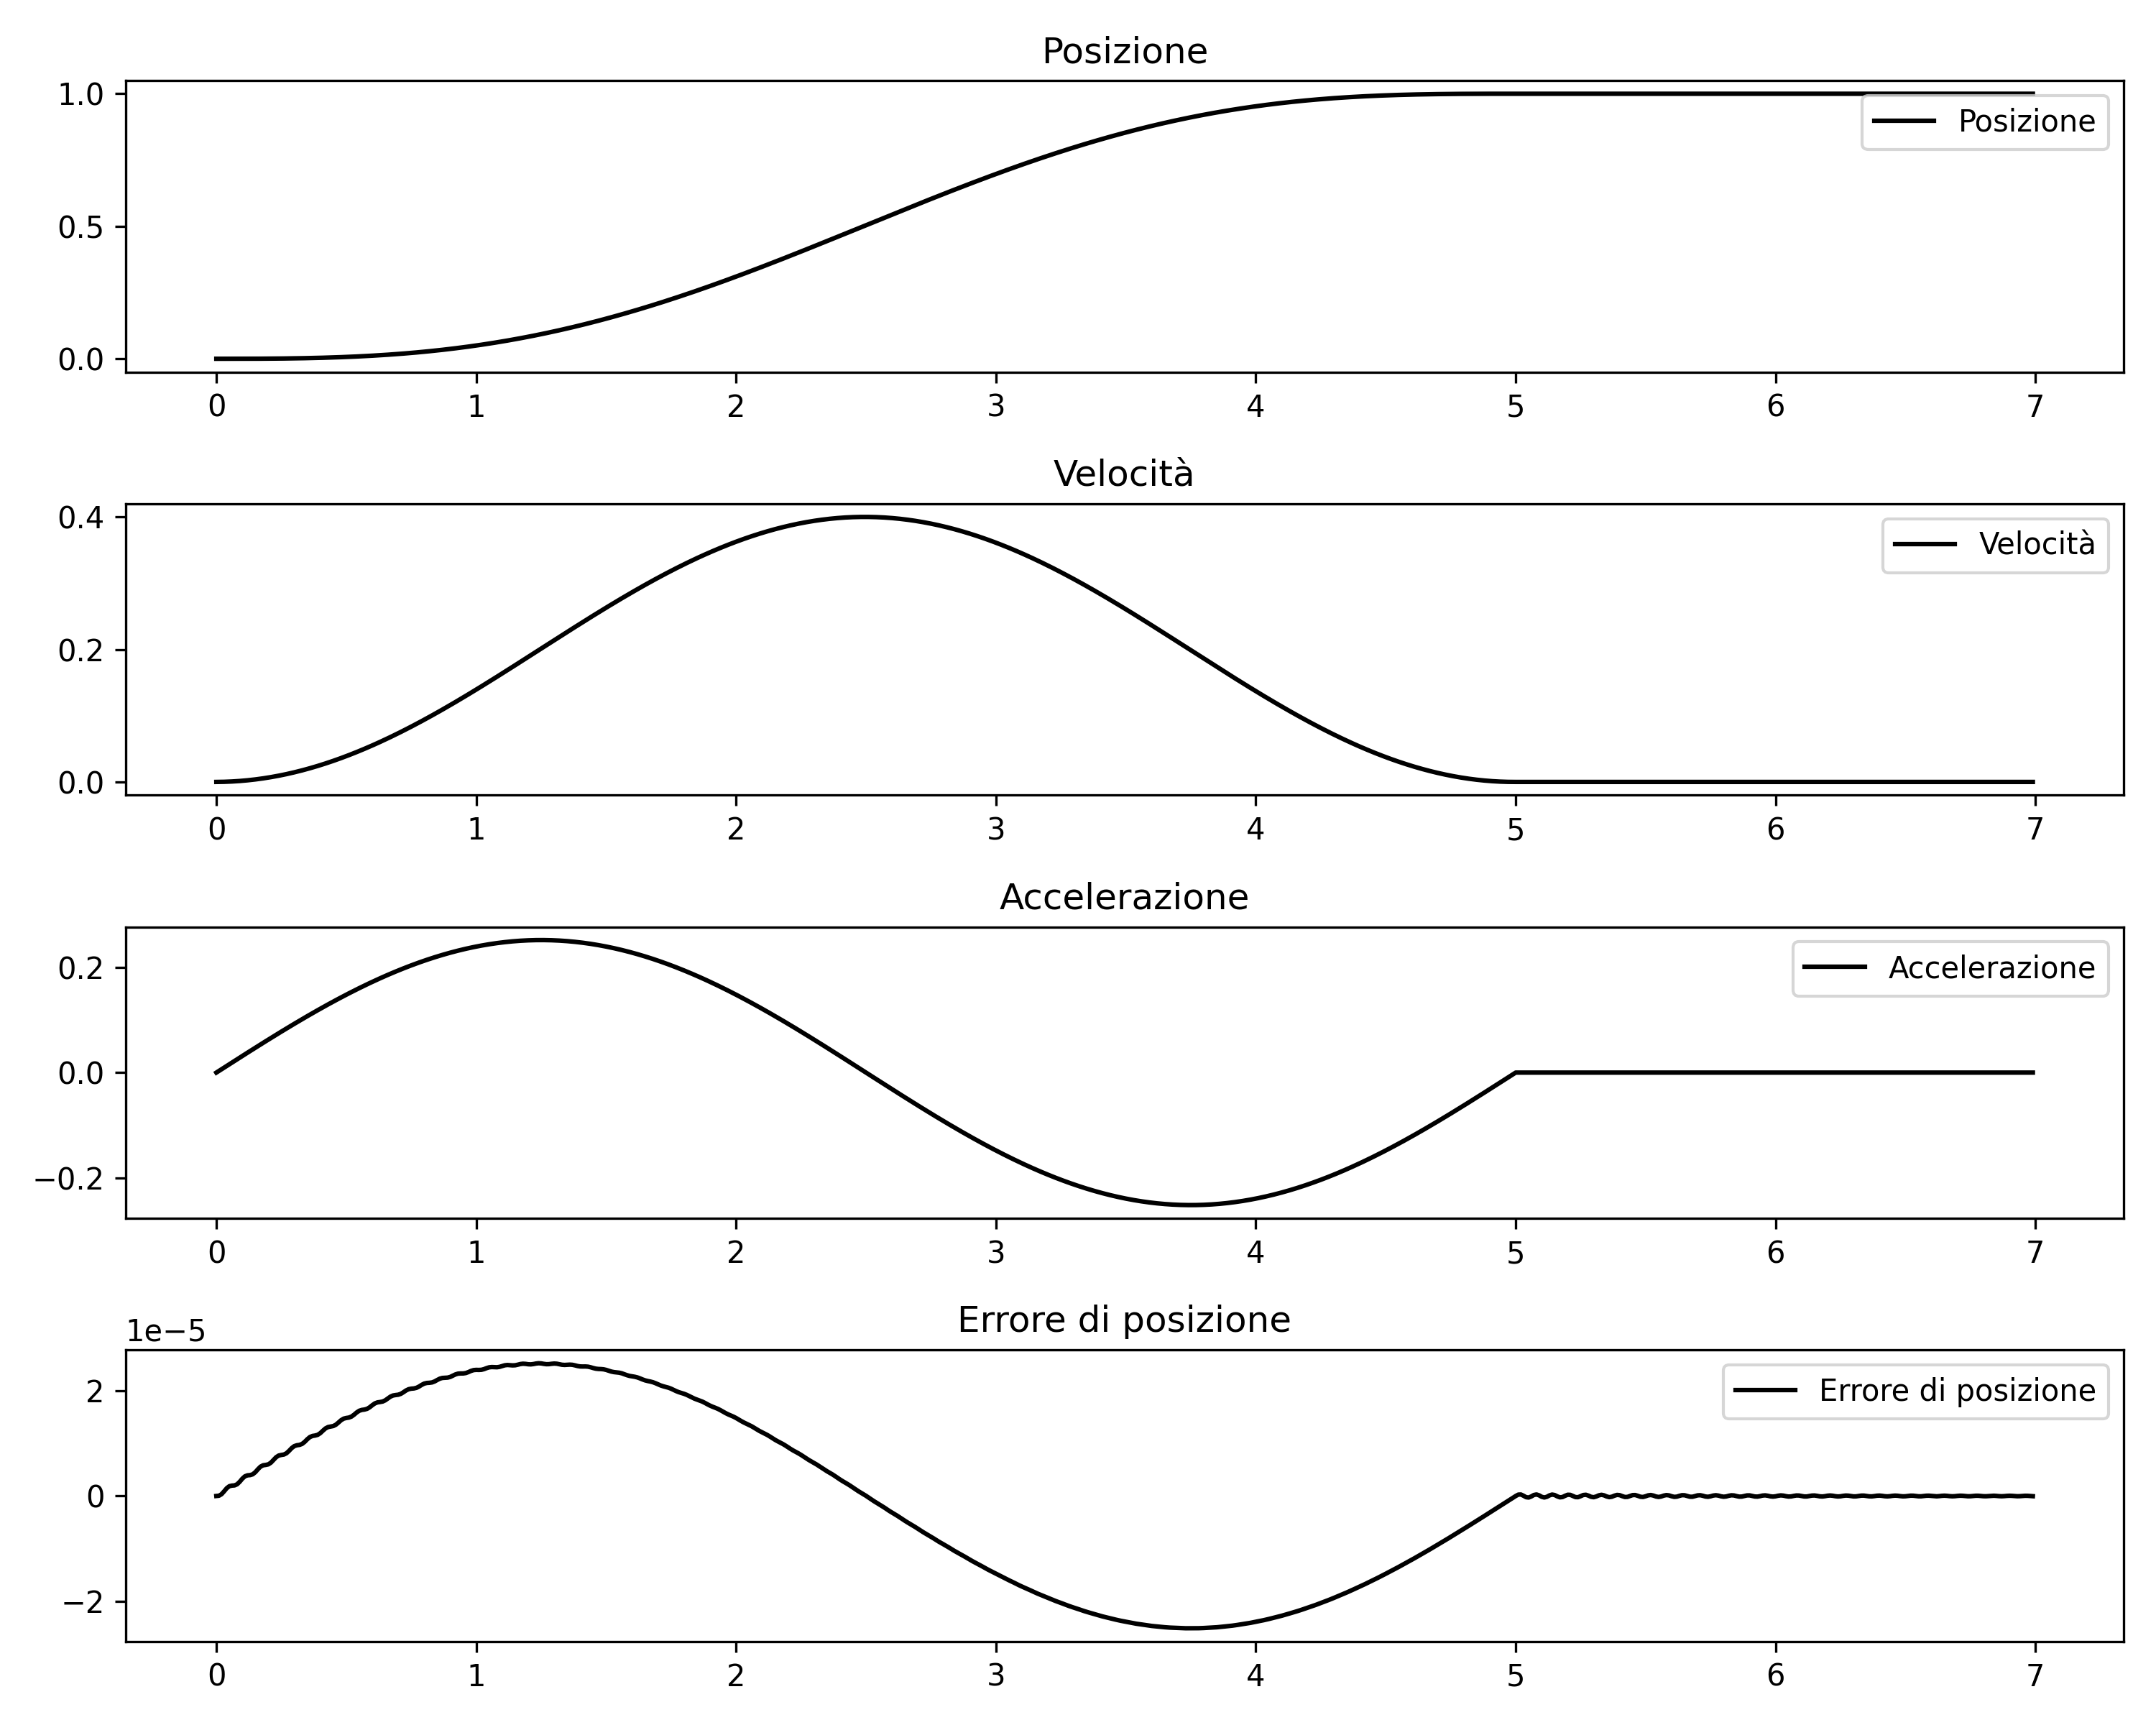
\includegraphics[width=0.45\textwidth]{Immagini/sinusoidale_colocato_v.png}
    \caption{Legge Armonica sx; Sinusoidale in accelerazione dx}
\end{figure}

\sottosottosezione{Rapporto di inerzia non nullo}
Per \(\rho > 0\) il controllo colocato permette di controllare indirettamente anche il carico.
Questo va diviso in più casi:
\begin{enumerate}
    \item Risonanza in "bassa" frequenza: \(\omega_p << \omega_{tv}, \omega_I\)
    \item Risonanza in "media" frequenza: \(\omega_z \simeq \omega_p \simeq \omega_{tv} \simeq \omega_I\)
    \item Risonanza in "alta" frequenza: \(\omega_z >> \omega_{tv}, \omega_I\)
\end{enumerate} 

\paragrafo{Risonanza in alta frequenza:}
Nel caso di risonanza in alta frequenza (circa un \(\times 2\) tra \(\omega_z\) e \(\omega_{tv},\omega_I\)) non possono essere misurate le oscillazioni dal trasduttore e il motore non può nè eccitare nè controllare le vibrazioni ad alta frequenza. Questo è il caso di un equivalente sistema rigido in cui le risonanza e antirisonanza sono filtrate da trasduttore e anello di corrente, perciò \(G_{vm}(s) \simeq \frac{1}{sJ}\) e l'anello aperto ha funzione di trasferimento \(L(s) \simeq \frac{1}{sJ} C_v K_T H_{trasd} W_I\).

\sottosottosezione{Rapporto di Inerzia non nullo, Risonanza in bassa frequenza}
Nel caso di risonanza in bassa frequenza (circa un \(\times 3;4\) tra \(\omega_z\) e \(\omega_{tv}, \omega_I\)) considero intanto il sistema senza gli effetti di trasduttore e anello di corrente che agiscono solo ad alta frequenza.
Per facilitare la realizzazione pratica si può considerare la relazione \(\omega_z < \omega_p << \omega_\pi\), perché la pulsazione di attraversamento si verifica, nel controllo colocato, per effetto di trasduttore e anello di corrente.

\paragrafo{Valutazione sulla catena chiusa:}
La funzione di trasferimento in catena chiusa è \(W_v(s) \simeq \frac{G_{vm}C_v K_T}{1+G_{vm}C_v K_T}\), i poli del sistema possono essere analizzati col luogo delle radici (i poli possono essere variati con il \(K_{pv}\)), mentre gli zeri del sistema sono legati a \(G_{vm}C_v\) che ha una coppia di zeri aventi \(\xi_z, \omega_z\), per cui l'antirisonanza della catena chiusa è la stessa di \(G_{vm}\) e uno zero reale \(s=-\frac{1}{T_{iv}}\).

\paragrafo{Con controllore PI:}
Abbiamo visto come il controllo di velocità convenga venire effettuato con controllore PI, di seguito il luogo delle radici in questo caso. A differenza del luogo delle radici con proporzionale si notano il polo nullo e lo zero sull'asse reale.

\begin{figure}[h]
    \centering
    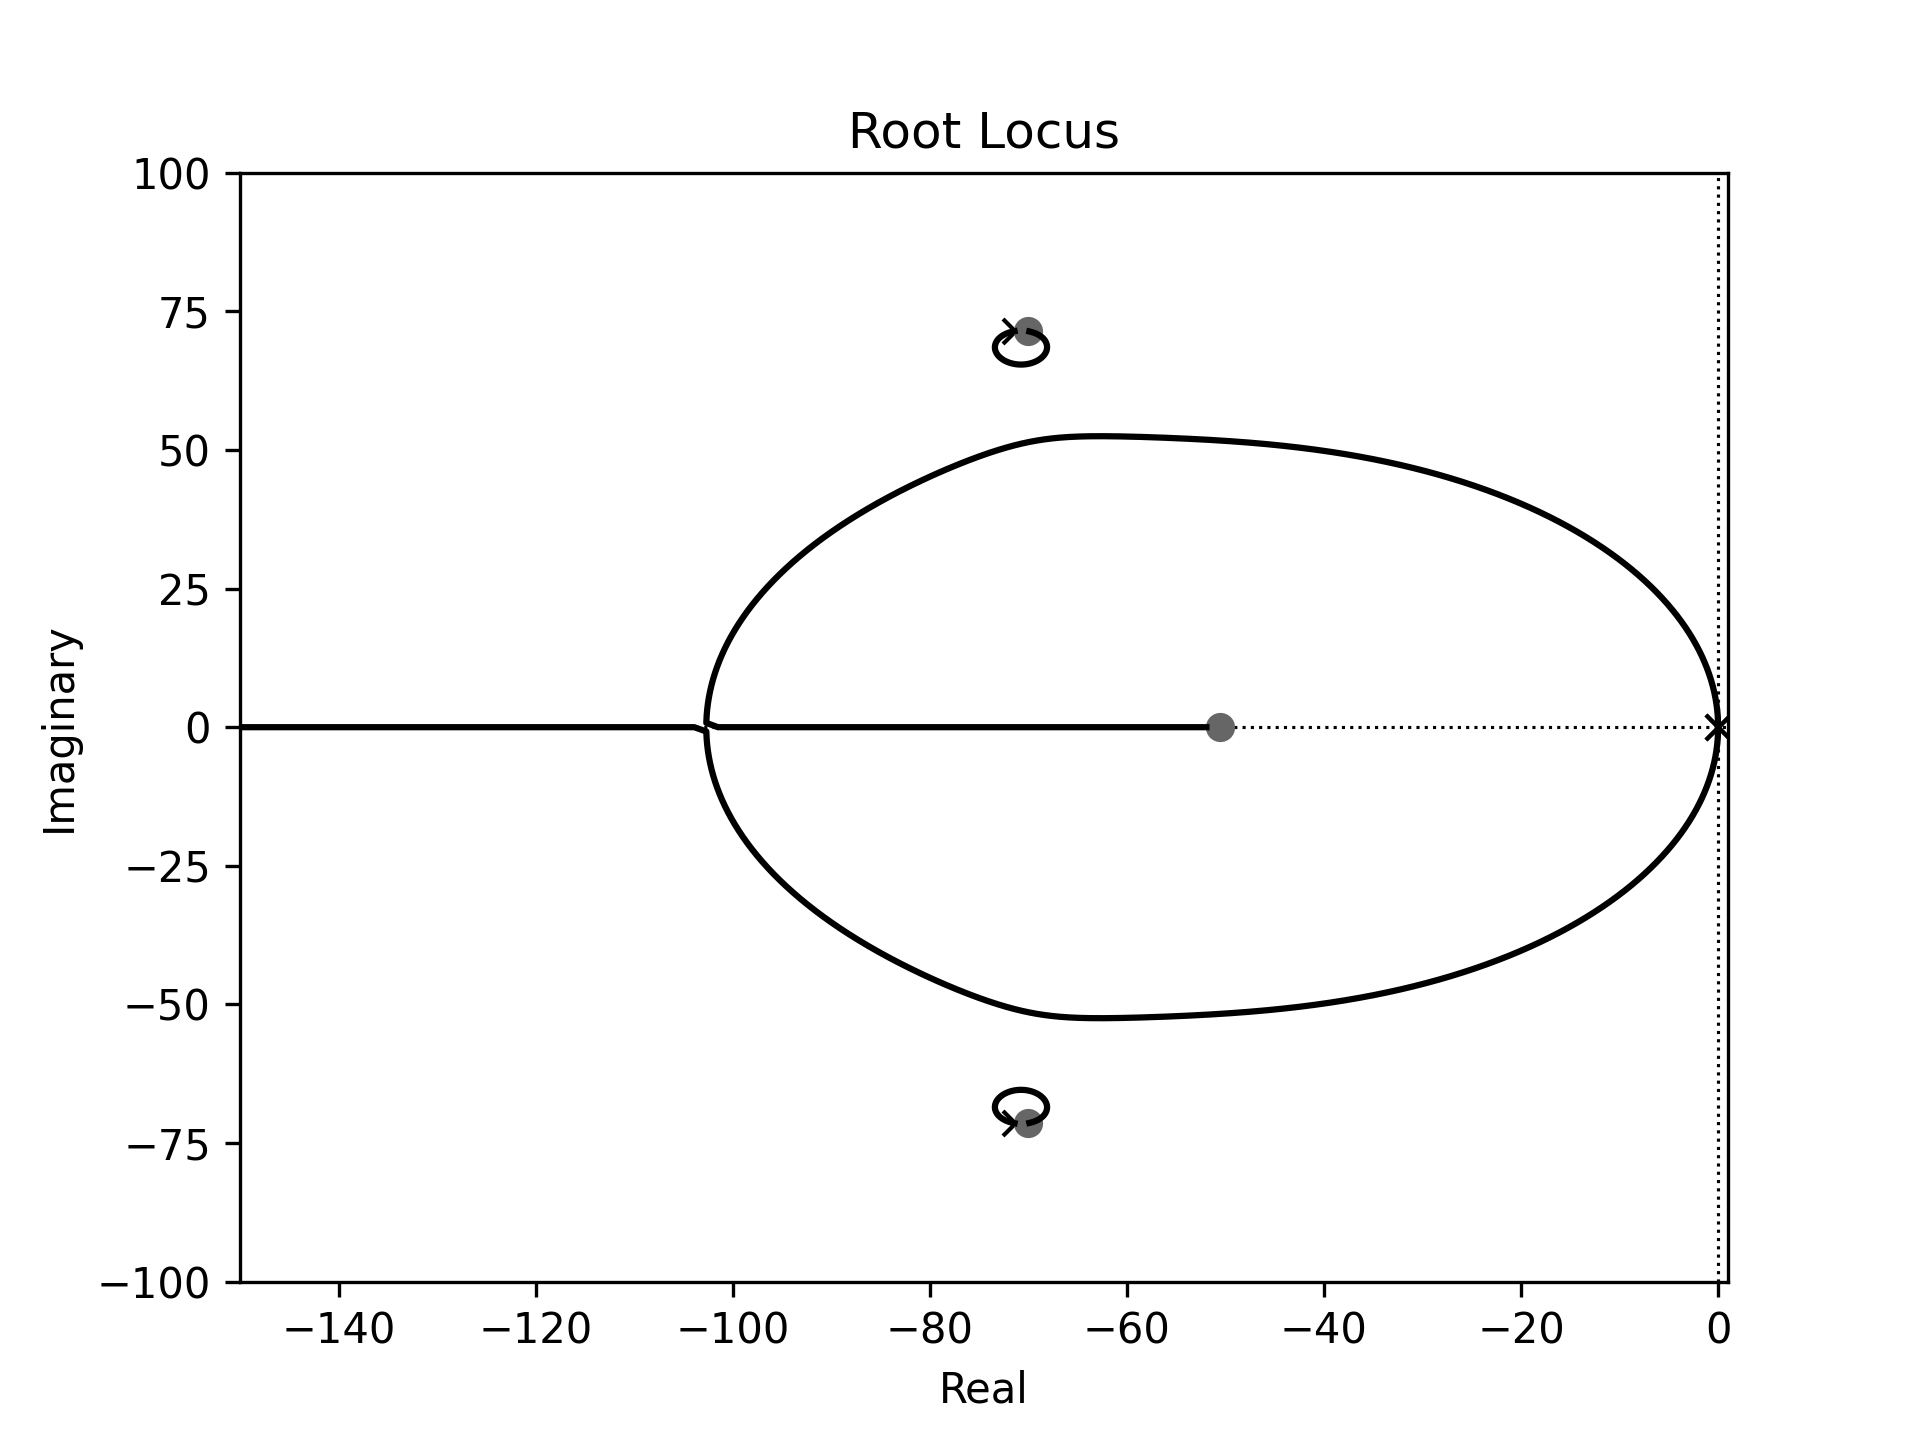
\includegraphics[width=0.4\textwidth]{Immagini/controllo_v_colocato_PI.png}
    \caption{Controllo Colocato con controllore PI}
\end{figure}

\paragrafo{Tipici approcci di progetto:}
Fissato \(\omega_{bv}^{des} \simeq [0.5\div 0.7]\omega_z\), calcolo, approssimando il sistema ad un sistema rigido, \(K_{pv} \simeq \frac{\omega_{bv}^{des} J}{K_T}\) e \(\frac{1}{T_{iv}} \simeq \frac{\omega_{bv}^{des}}{4 \xi_{des}^2}\) con smorzamento del polo del sistema a catena chiusa \(\xi_{des} \geqslant 1\) (perché non conviene rischiare avendo trasmissione elastica).
Alternativamente è possibile partire considerando il luogo delle radici, e cercare \(K_{pv}\) tale che siano massimizzati \(\xi_{poli}\) o \(\mathbb{R}(\text{poli})\).
I due metodi portano a \(K_{pv}\) paragonabili e nella zona di ottimo.
Tenendo a mente che rimane da garantire \footnote{Vedi \ref{Teq} per condizioni per sistema con trasmissione rigida.} \(\omega_{bv} > \frac{\frac{1}{T_{eq}}}{4\xi^2}\).

\paragrafo{Valutazioni sul carico:}
Il picco di risonanza della trasmissibilità "compensa" il picco di antirisonanza di \(W_v\), lato carico si ottiene un \(\omega_{bv}\) maggiore.
Bisogna quindi prestare attenzione a utilizzare guadagni troppo elevati perché il motore potrà beneficiarne, ma questo potrebbe portare ad avere una eccessiva compensazione, da parte della trasmissibilità, lato carico, causando di picchi di risonanza.

\begin{figure}[h]
    \centering
    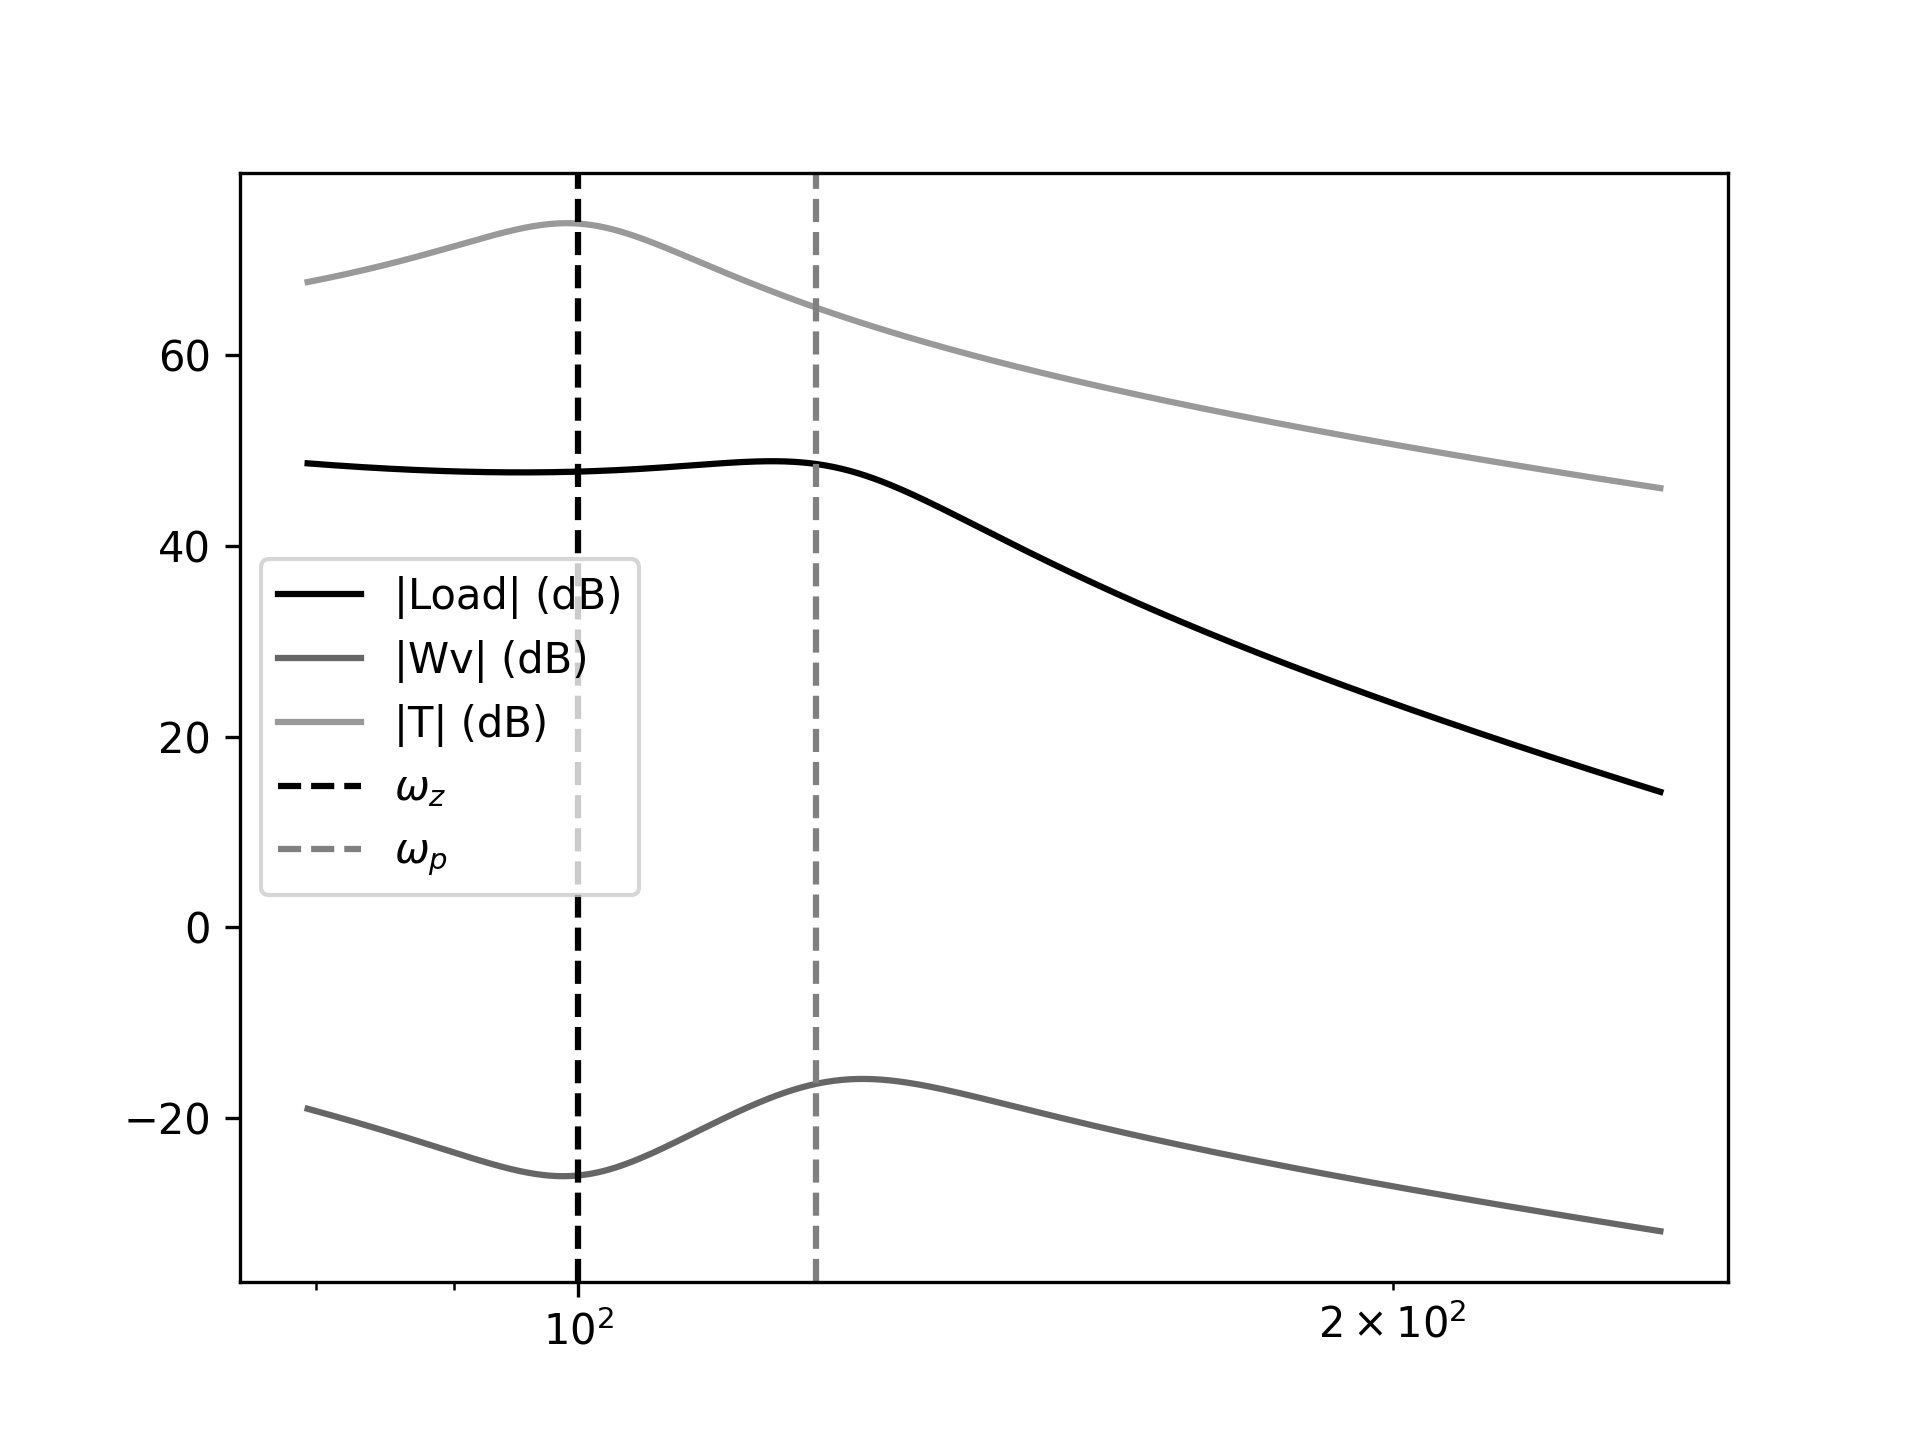
\includegraphics[width=0.45\textwidth]{Immagini/colocato_v_lato_carico.png}
    \caption{Controllo Colocato lato carico}
\end{figure}

\paragrafo{Risposta al gradino per vari guadagni:}
La risposta al gradino per un sistema che abbia impostato un guadagno \(K_{pv,2}\) "ottimo" \footnote{Nè troppo elevato, per cui lato carico si ottenga picco di risonanza per eccesso di compensazione, nè troppo ridotto, per cui si ottiene una bassa banda passante} ha una sovraelongazione dovuta allo zero a causa della scelta del gradino come legge di moto, ma carico e motore mantengono andamenti simili.
La risposta al gradino per un sistema che abbia impostato un guadagno \(K_{pv,3}\) "troppo elevato" vede grandi oscillazioni sia al motore sia al carico, non seguono nemmeno andamenti simili, perché sono peggiori al carico.

% inserire immagine di risposta al gradino \rho = 4 \xi = 0.7

\sottosottosezione{Risonanza in media frequenza}



% meccanica delle vibrazioni, aggiungere parte su decremento logaritmico